\documentclass{jsarticle}
\usepackage{amsmath}
\usepackage{url}
\usepackage{graphicx}
\usepackage{here}
\usepackage{listings}
\lstset{
    basicstyle={\ttfamily\small}, %書体の指定
    frame=tRBl, %フレームの指定
    framesep=10pt, %フレームと中身(コード)の間隔
    breaklines=true, %行が長くなった場合の改行
    linewidth=12cm, %フレームの横幅
    lineskip=-0.5ex, %行間の調整
    tabsize=2 %Tabを何文字幅にするかの指定
}

\begin{document}
\begin{titlepage}
    \begin{center}
        \vspace*{12pt}
        {\huge 計算機科学実験及び演習2(SPICEシミュレーション)}
        \vspace{12pt}\\
        {第2回}
        \vspace{60pt}\\
        {締め切り : 12月24日}
        \vspace{12pt}\\
        {提出日 : 12月24日}
    \end{center}

    \vspace{400pt}
    \begin{flushright}
       {\large 学籍番号: 1029300562\\
        氏名: 新山公太(にいやまこうた)}
    \end{flushright}

    
\end{titlepage}

\section{課題1}
\subsection{微分回路}
\subsubsection{パラメータの値}
\begin{flushleft}
抵抗: $10k\Omega$\\
コンデンサの容量: $510pF$
\end{flushleft}

\subsubsection{手順}
まずは配布された資料の図2: SPICE回路記述例を参考にして、微分回路を構成した。そしてインタラクティブに
操作して時定数を求めるのが面倒だったので、回路記述ファイル内に.controlと.endcでコマンドを埋め込んだ。配布資料に書いてあったmeasコマンドについてリファレンスで調べて見たところ、パラメータがある値をとるときの別のパラメータの値を取得できたり、その値を複数回とるときには何回目かを指定できたりすることがわかった。
したがってまずplotされた図を見たところ$time=100.5u$の時に測定する電圧は最大値を取ることがわかったので、measコマンドでtimeが上の時の電圧を求めて、次にその値の立ち下り$37\%$の所の電圧となるときのtimeを求めた。具体的にはletコマンドを使って新しく変数を定義して、その変数をmeasコマンドの中で使った。詳しくは添付のコードを参照されたい。
以下に回路図を示す。
\begin{figure}[H]
    \centering
    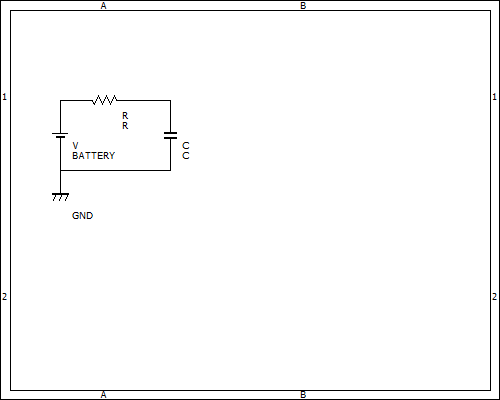
\includegraphics[bb=0 0 500 400]{ex1_dif.png}
    \caption{微分回路の回路図}
\end{figure}

\subsubsection{結果}
\begin{equation}
    \tau = 5.5707 \cdot 10^{-6} s
\end{equation}
理論値は、$\tau = 5.1 \cdot 10^{-6} s$であるので、この結果は正確に正しいとは言えなさそうである。このことについてはあとで考察したい。

\subsubsection{考察}
まず時定数が理論値と一致しないことについて考えたい。そもそもコンデンサは最初は充電されていないのでグラフにおいて$V$の最大値は$2.5V$となるはずである。しかし、実際には約$2.27V$しかない。これは入力の電圧が理論上では瞬時に切り替わると仮定しているが実際にはそうはいかないことによると思われる。電圧が上昇していっている途中にもコンデンサは充電されており、さらに測定している電圧は入力の電圧より大きくは絶対にならないので比較的強く影響を受けてしまう。この最大電圧のずれにより、立ち下がり$37\%$の点もずれてしまったことで理論値から外れた測定値が得られたのだと思う。この入力の遅延による時定数のずれは前回オシロスコープを使って実際に測定したときには考慮していなかった部分であるので、今回の実験でこういった影響があることを確認できてよかった。
ちなみに入力が$100\mu s$で変わるとして、そこから$5.1\mu s$後の$V$の値を$0.37$で割ったところ、$2.489774$という値が得られたので、今回は電圧の最大値を$2.5V$と決めつけてしまったほうが良い結果が得られたと思う。

\begin{figure}[H]
    \hspace{50pt}
    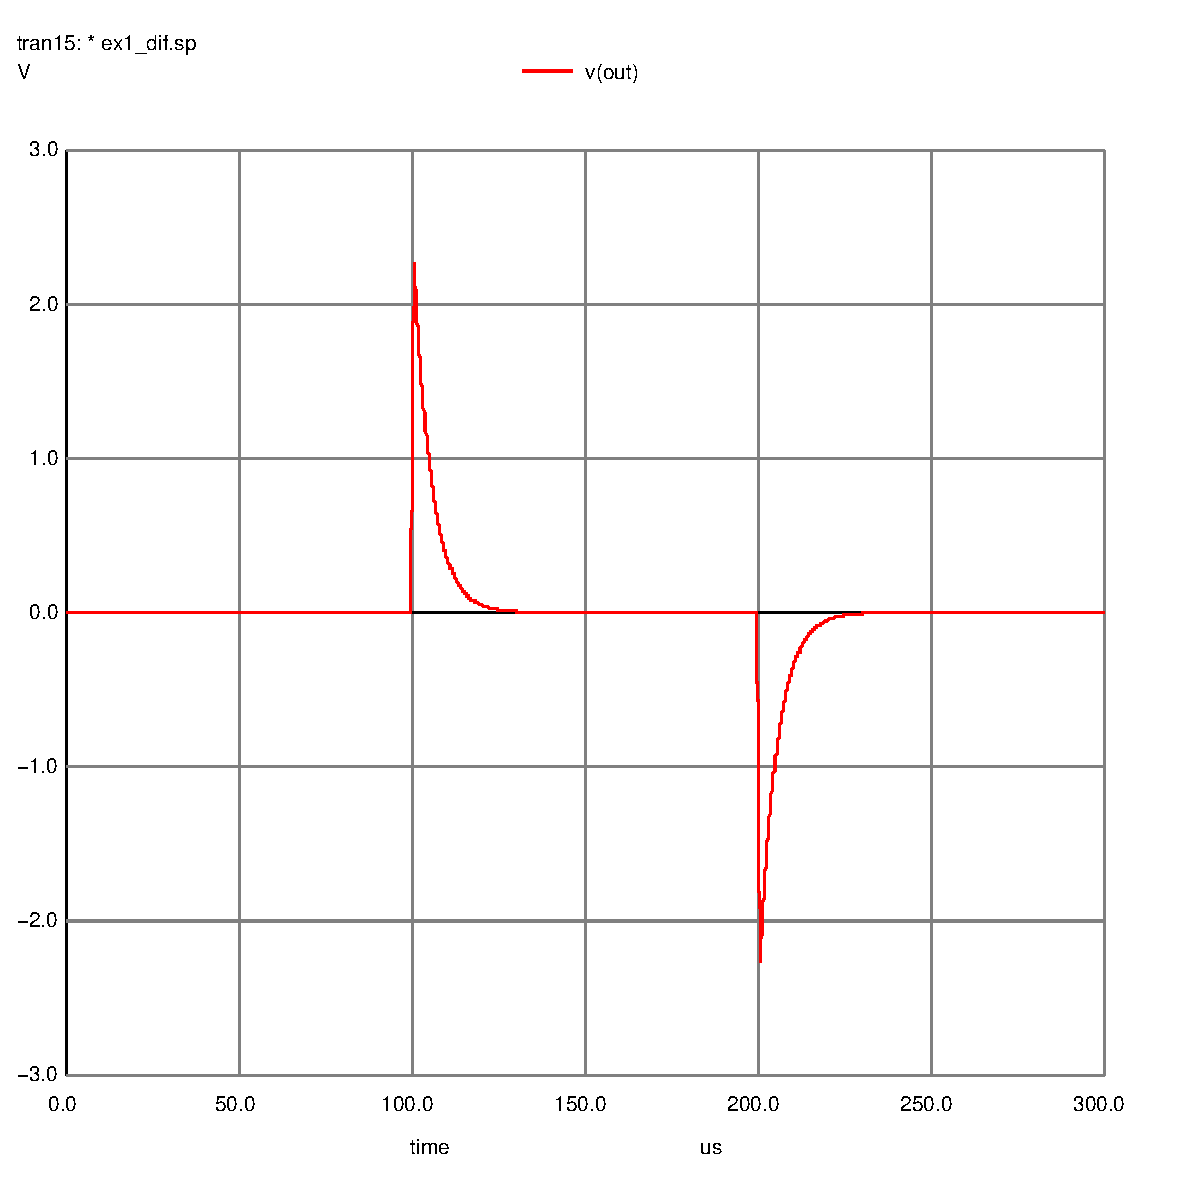
\includegraphics[scale=0.8]{ex1_dif.ps}
    \vspace{30pt}
    \caption{微分回路の$V-t$グラフ}
\end{figure}

\subsection{積分回路}

\subsubsection{パラメータの値}
\begin{flushleft}
抵抗: $10k\Omega$\\
コンデンサの容量: $510pF$
\end{flushleft}

\subsubsection{手順}
微分回路と同じようにしたが今回異なるのは、振幅が$2.5V$となっている点である。
また、時定数として使われる値も変わっていて積分回路では立ち上がりが$63\%$となった時間となっている。
以下に回路図を示す。
\begin{figure}[H]
    \centering
    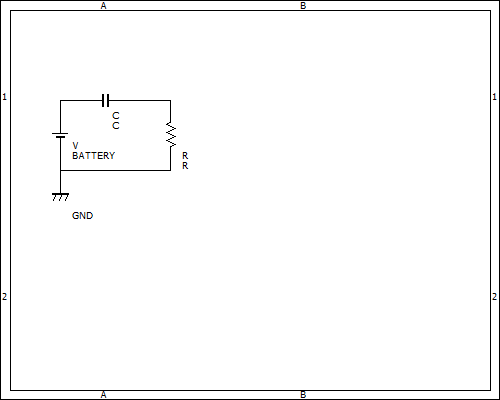
\includegraphics[bb=0 0 500 400]{ex1_integral.png}
    \caption{積分回路の回路図}
\end{figure}

\subsubsection{結果}
\begin{equation}
    \tau = 5.7091 \cdot 10^{-6} s 
\end{equation}
理論値では$\tau = 5.1 s$となるので積分回路も正確な値からのずれが少しだが生じる。微分回路の時と同様にこれについて考察したい。また、微分回路と比べてなぜ誤差が小さいのかについても考えたい。

\subsubsection{考察}
まず積分回路では振幅が$2.5V$となっている。コンデンサは入力が切り替わる非常に短い時間の間にも充電されるので、微分回路ではとりうる最大の電圧に影響を及ぼしていた。積分回路でも入力の遅延による影響を受けてコンデンサの充電が入力の遅延の間にも行われるが、コンデンサには電荷がゆっくり溜まっていくので、入力の遅延の影響が小さいと考えられる。この影響によって確かに立ち上がり$63\%$の点はずれるがそのずれは微分回路の時よりも小さなものとなる。
ちなみに、積分回路の時定数は微分回路で振幅を$2.5V$として考えた時の時定数と一致することが確認できた。
\begin{figure}[H]
    \hspace{50pt}
    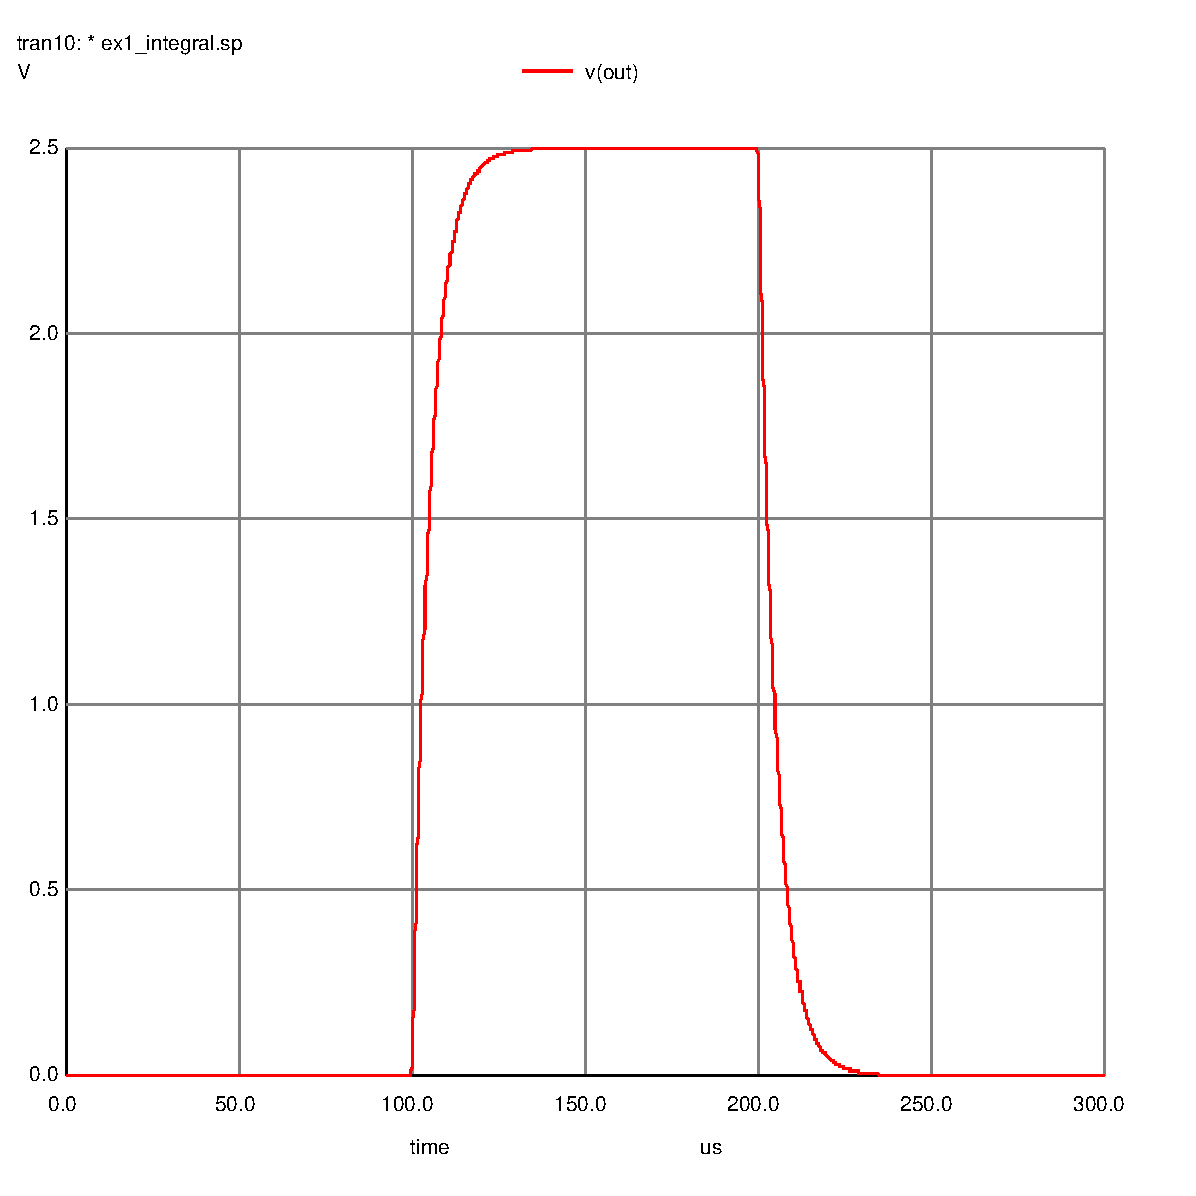
\includegraphics[scale=0.8]{ex1_integral.ps}
    \vspace{30pt}
    \caption{積分回路のグラフ}
\end{figure}


\section{課題2}
課題2-1では立ち上がりと立下りの遅延時間をそれぞれ評価する。
課題2-2において種々の論理ゲートを負荷とした回路での遅延の評価では、立ち上がりの遅延時間と立下りの遅延時間の平均を基準として評価することにする。

\subsection{負荷がコンデンサの場合}
\subsubsection{手順}
配布された資料の図4: インバータの動作確認にある通りの回路を作成する。
課題1の時と同様に回路記述ファイル内にコマンドを埋め込んだ。具体的には、measコマンドでv(out)が$1.25V$を取る時のtimeを取得した。これは今回は立ち上がりと立下りの2回あるのでCROSSオプションで何回目の交差かを指定した。
なおコンデンサの容量は資料で指定された通り$30fF$とした。
以下に回路図を示す。
\begin{figure}[H]
    \centering
    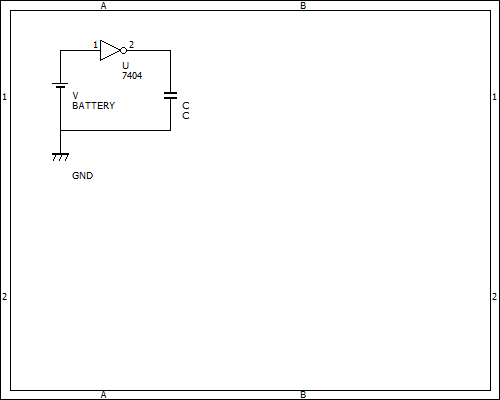
\includegraphics[bb=0 0 500 400]{ex2_1.png}
    \caption{コンデンサを負荷とした時の回路図}
\end{figure}
\subsubsection{結果}
\begin{flushleft}
立ち上がりの遅延時間: $8.12 \cdot 10^{-11} s$\\
立下りの遅延時間: $2.263 \cdot 10^{-10} s$
\end{flushleft}

\begin{figure}[H]
    \hspace{50pt}
    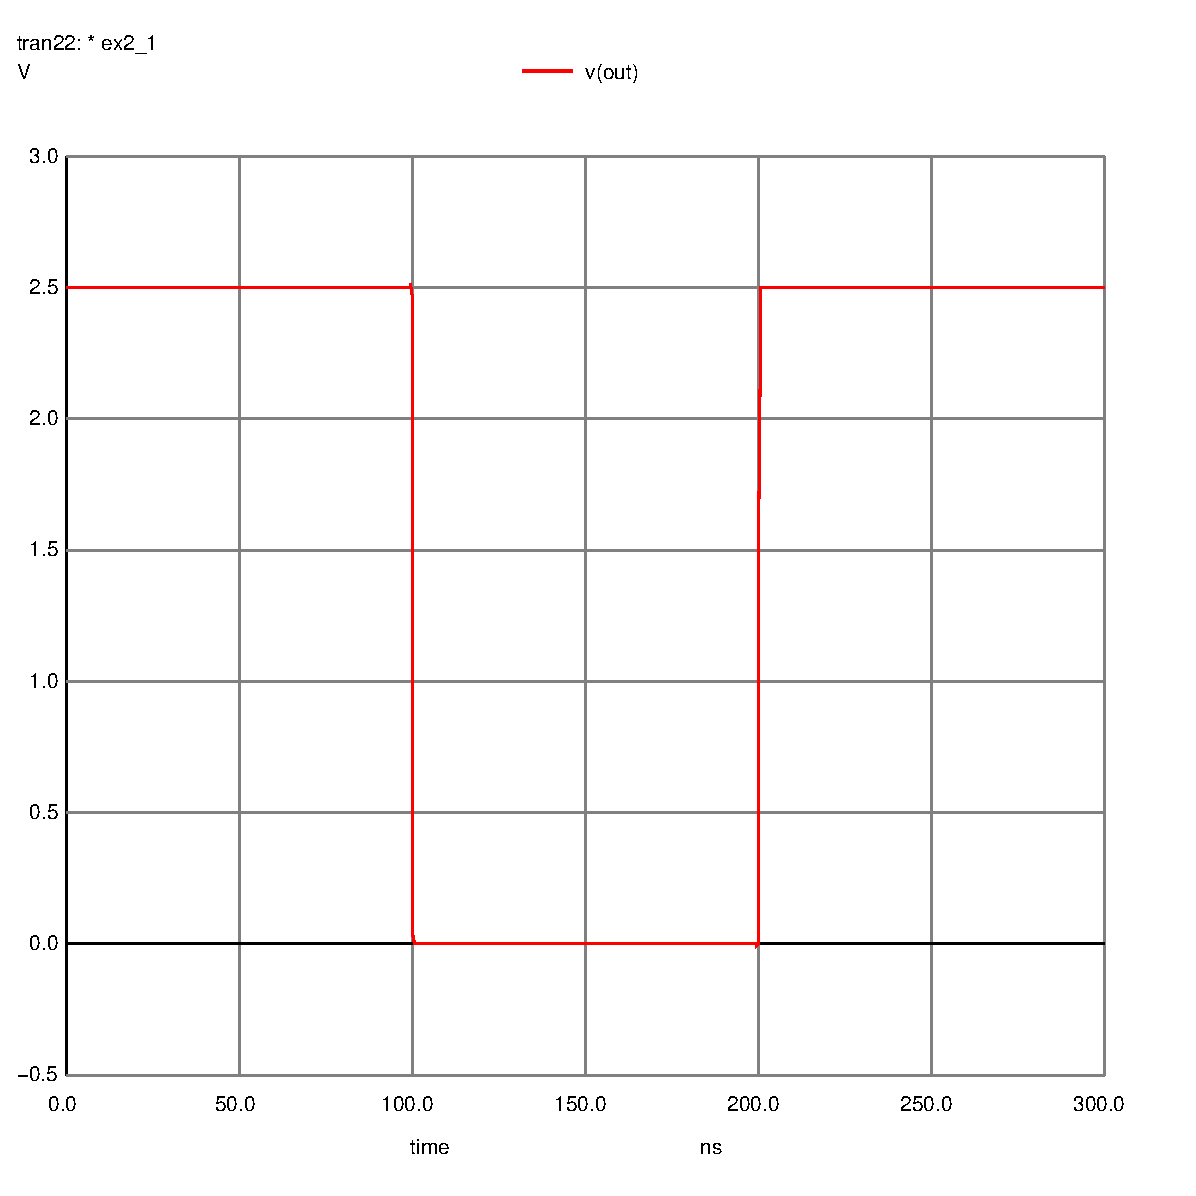
\includegraphics[scale=0.8]{ex2_1.ps}
    \vspace{30pt}
\end{figure}

\subsection{課題2-2}
課題2-1の回路の負荷として様々な論理素子を接続して遅延時間を測定した。

\subsubsection{負荷がインバータの場合}
以下に回路図を示す。
\begin{figure}[H]
    \centering
    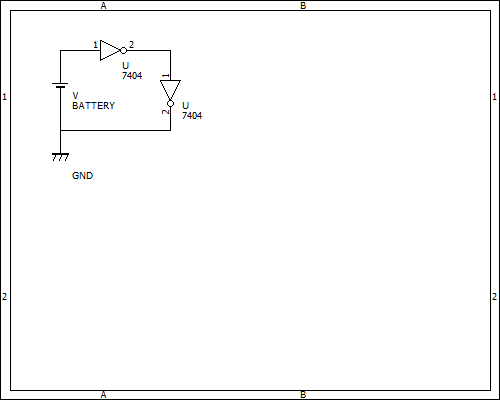
\includegraphics[bb=0 0 500 400]{ex2_2_inv.png}
    \caption{インバータを負荷とした時の回路図}
\end{figure}

\begin{flushleft}
    立ち上がり: $3.86 \cdot 10^{-11}$\\
    立下り: $1.846 \cdot 10^{-10}$
\end{flushleft}
\begin{figure}[H]
    \hspace{50pt}
    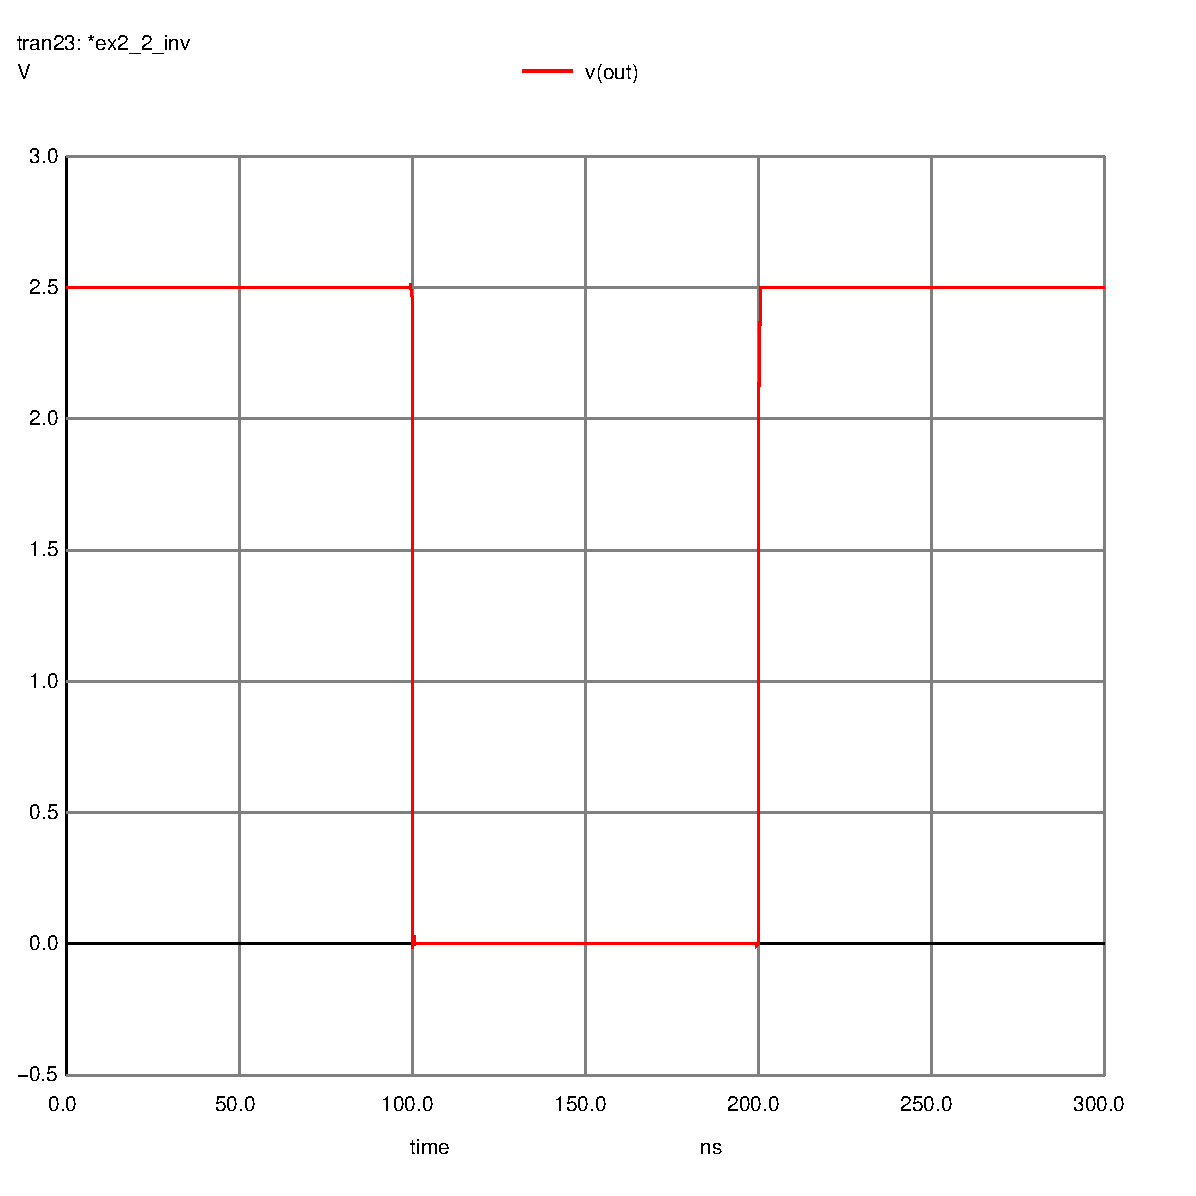
\includegraphics[scale=0.8]{ex2_2_inv.ps}
    \vspace{30pt}
    \caption{インバータを負荷として接続}
\end{figure}

\subsubsection{負荷がインバータ2つの場合}
\begin{figure}[H]
    \centering
    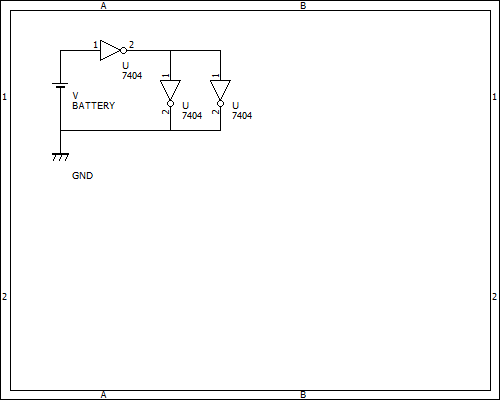
\includegraphics[bb=0 0 500 400]{ex2_2_double_inv.png}
    \caption{インバータ2つを負荷とした時の回路図}
\end{figure}

\begin{flushleft}
    立ち上がり: $8.04\cdot 10^{-11}$\\
    立ち下り: $2.249 \cdot 10^{-10}$
\end{flushleft}
\begin{figure}[H]
    \hspace{50pt}
    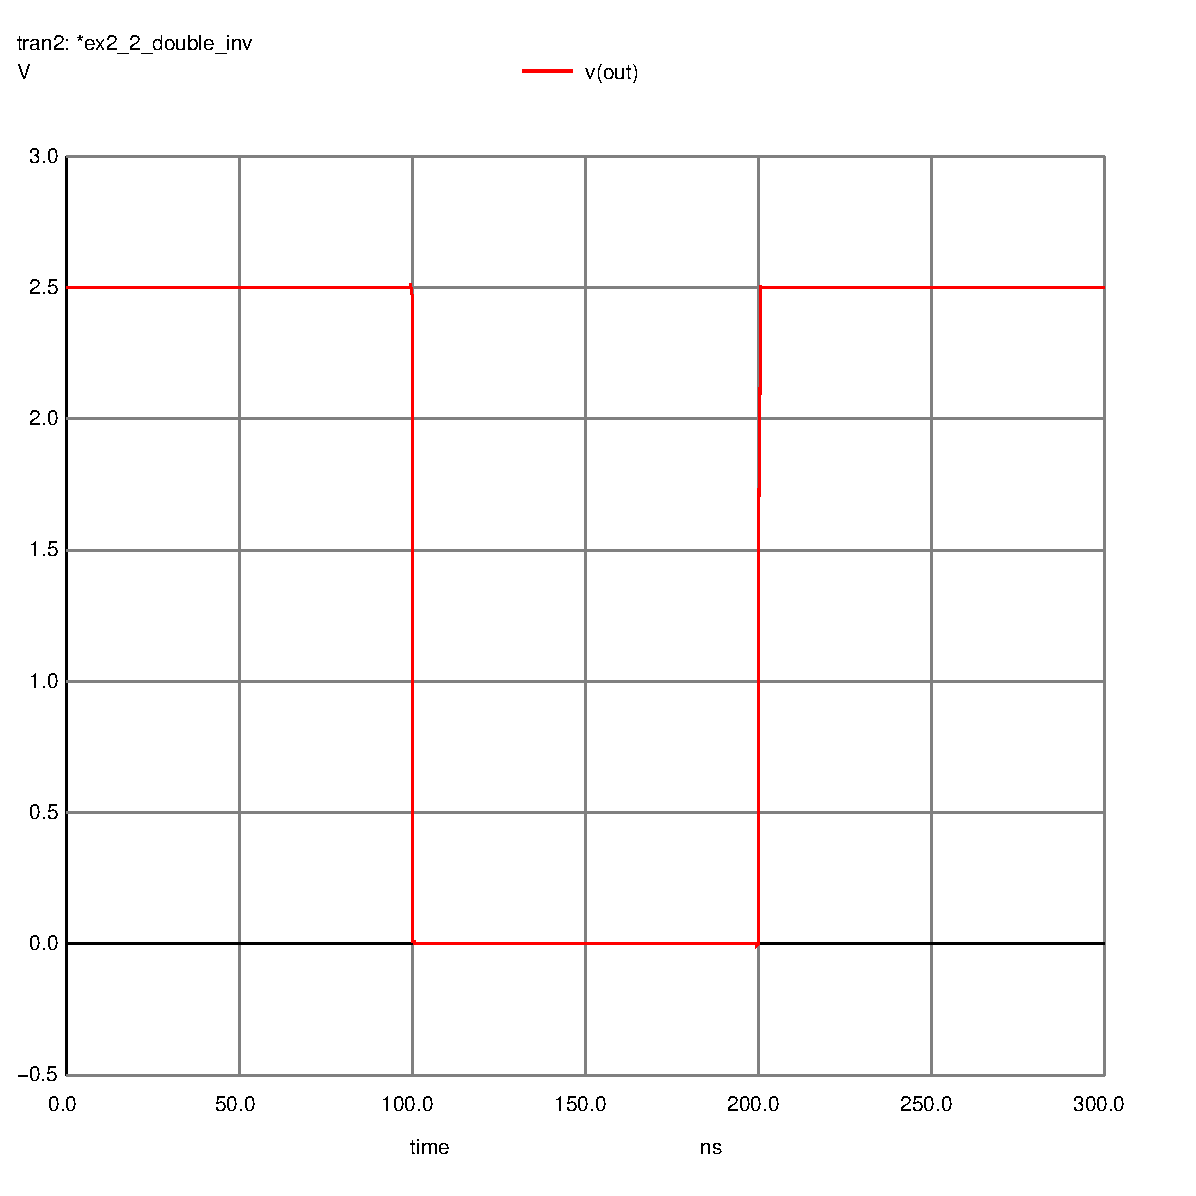
\includegraphics[scale=0.8]{ex2_2_double_inv.ps}
    \vspace{30pt}
    \caption{インバータ2つを負荷として接続}
\end{figure}


\subsubsection{負荷がインバータ3つの場合}
\begin{figure}[H]
    \centering
    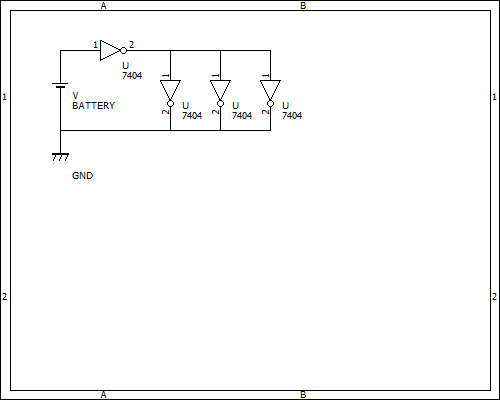
\includegraphics[bb=0 0 500 400]{ex2_2_triple_inv.png}
    \caption{インバータ3つを負荷とした時の回路図}
\end{figure}

\begin{flushleft}
    立ち上がり: $1.168 \cdot 10^{-10}$\\
    立ち下り: $2.673 \cdot 10^{-10}$
\end{flushleft}
\begin{figure}[H]
    \hspace{50pt}
    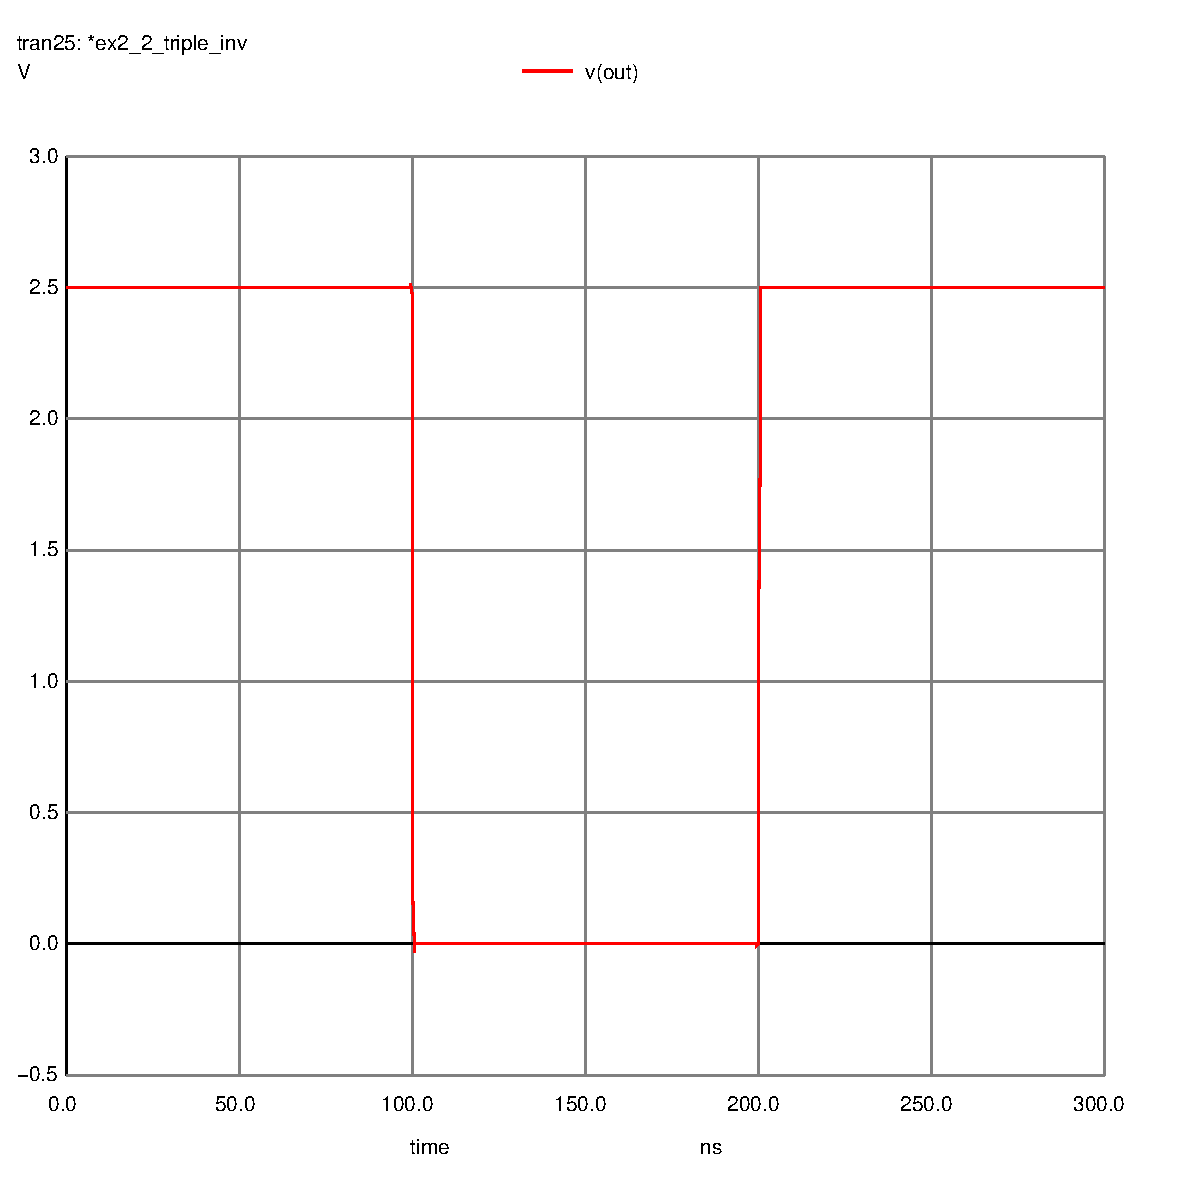
\includegraphics[scale=0.8]{ex2_2_triple_inv.ps}
    \vspace{30pt}
    \caption{インバータ3つを負荷として接続}
\end{figure}

\subsubsection{負荷がサイズ2倍のインバータの場合}
\begin{figure}[H]
    \centering
    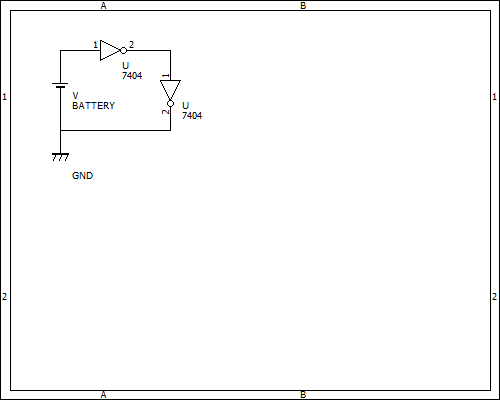
\includegraphics[bb=0 0 500 400]{ex2_2_inv.png}
    \caption{サイズ2倍インバータを負荷とした時の回路図}
\end{figure}

\begin{flushleft}
    立ち上がり: $8.01 \cdot 10^{-11}$
    立ち下り: $2.243 \cdot 10^{-10}$
\end{flushleft}
\begin{figure}[H]
    \hspace{50pt}
    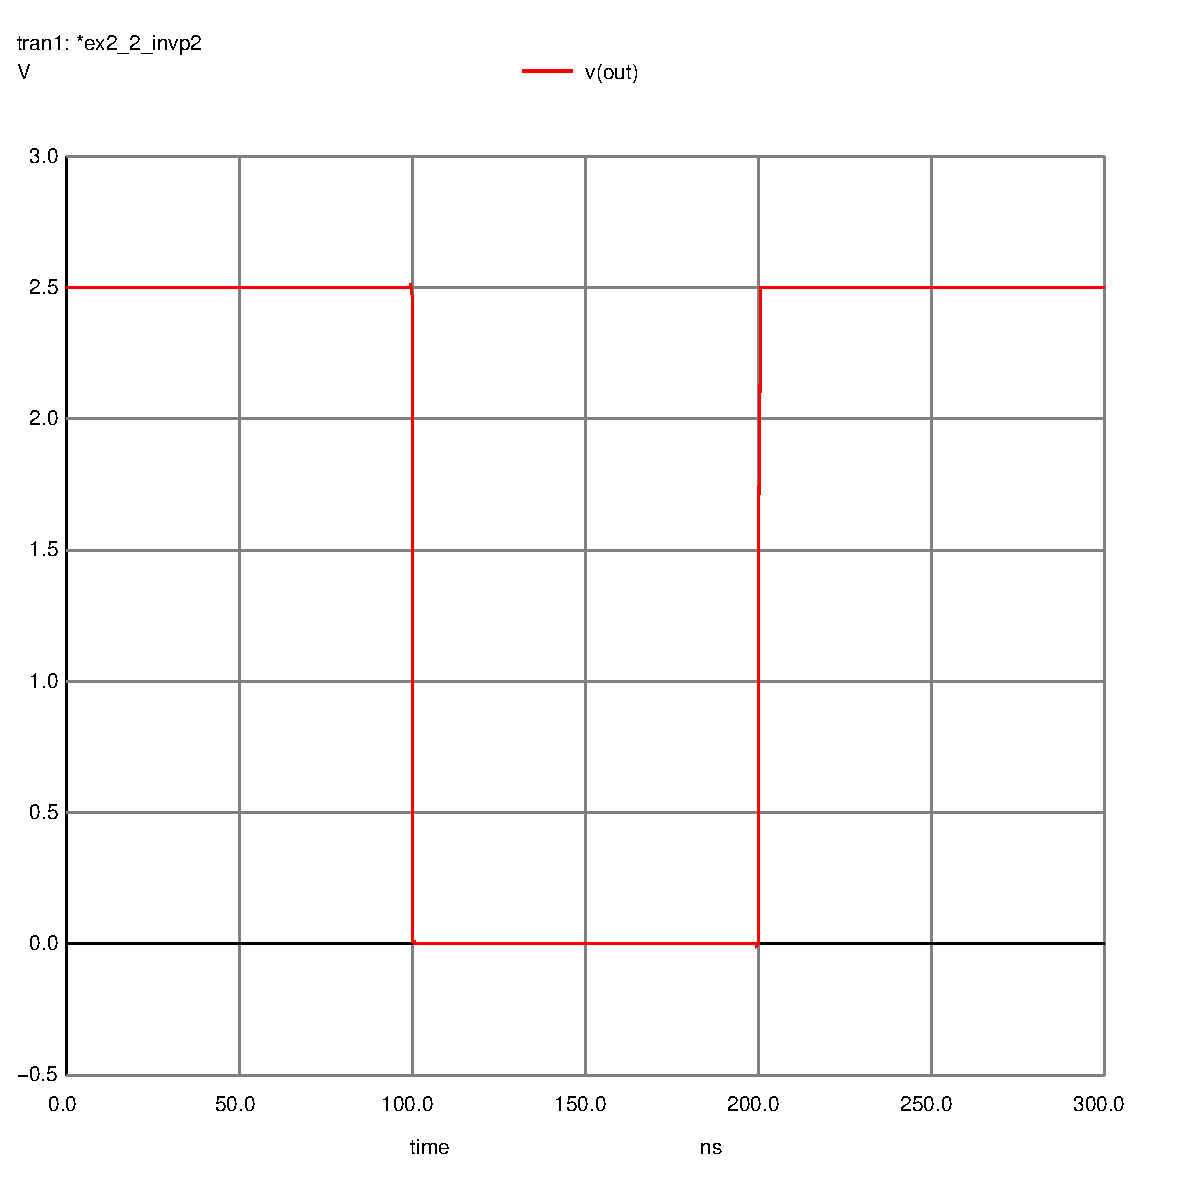
\includegraphics[scale=0.8]{ex2_2_invp2.ps}
    \vspace{30pt}
    \caption{サイズ2倍のインバータを負荷として接続}
\end{figure}

\subsubsection{負荷がサイズ4倍のインバータの場合}
\begin{figure}[H]
    \centering
    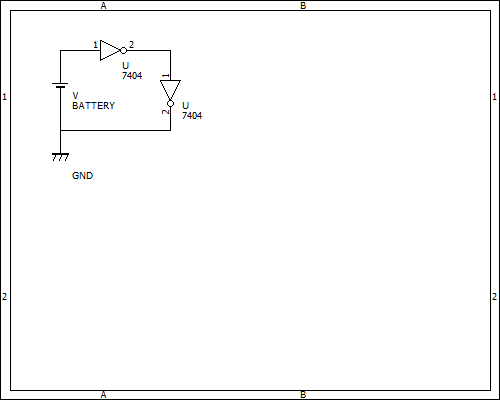
\includegraphics[bb=0 0 500 400]{ex2_2_inv.png}
    \caption{サイズ4倍インバータを負荷とした時の回路図}
\end{figure}

\begin{flushleft}
    立ち上がり: $1.525 \cdot 10^{-10}$\\
    立ち下り: $2.964 \cdot 10^{-10}$
\end{flushleft}
\begin{figure}[H]
    \hspace{50pt}
    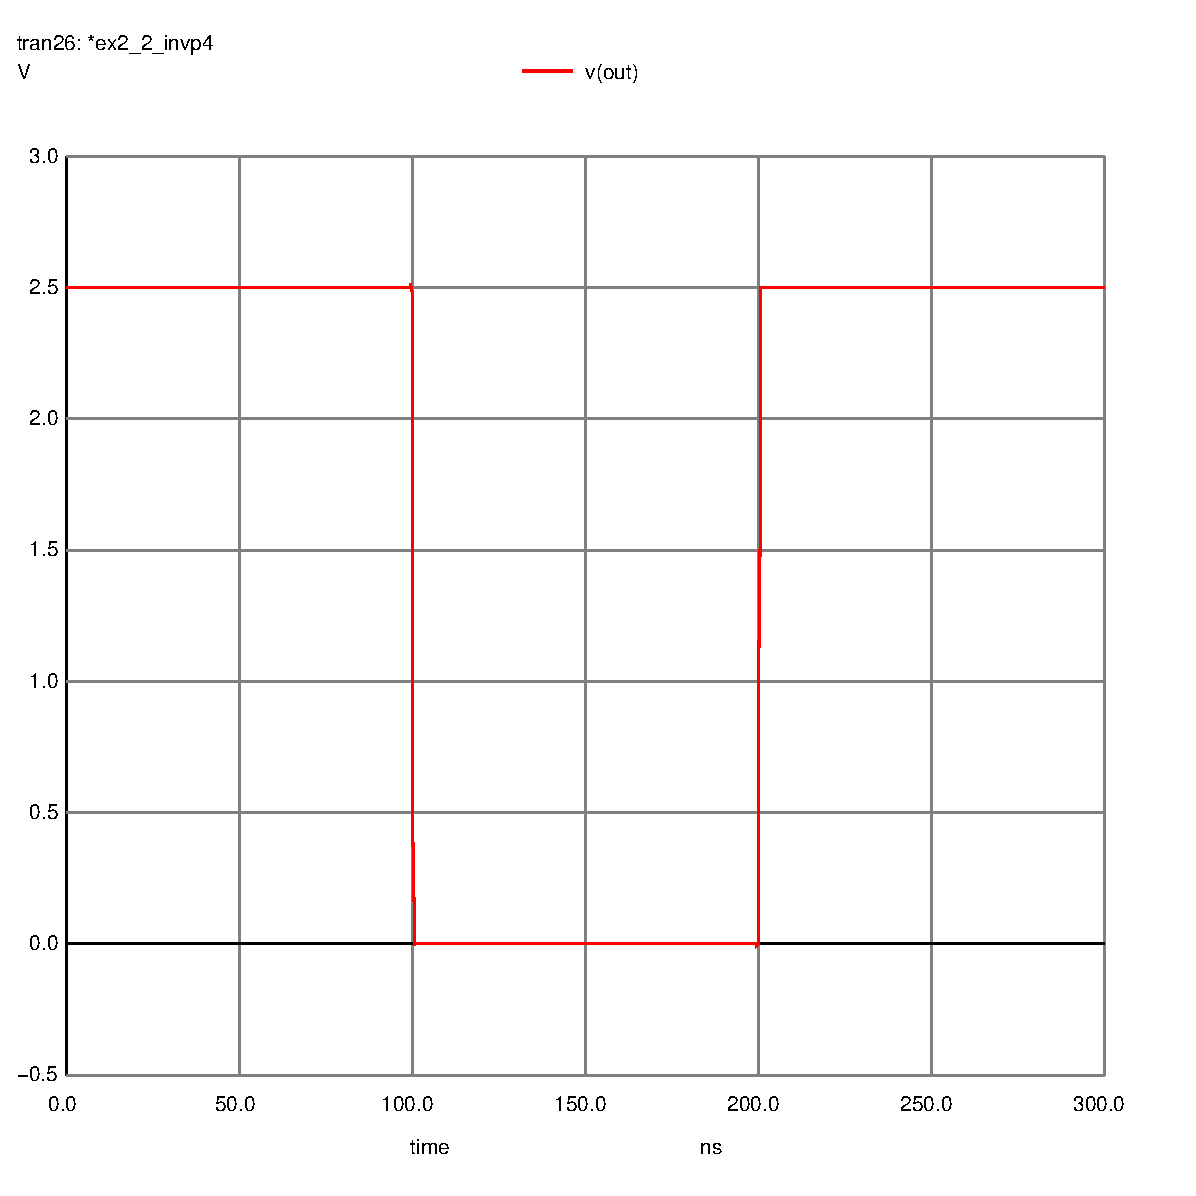
\includegraphics[scale=0.8]{ex2_2_invp4.ps}
    \vspace{30pt}
    \caption{サイズ4倍のインバータを負荷として接続}
\end{figure}

\subsubsection{負荷がサイズ8倍のインバータの場合}
\begin{figure}[H]
    \centering
    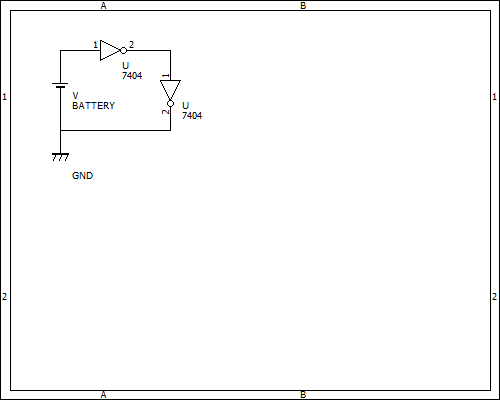
\includegraphics[bb=0 0 500 400]{ex2_2_inv.png}
    \caption{サイズ8倍インバータを負荷とした時の回路図}
\end{figure}

\begin{flushleft}
    立ち上がり: $2.593 \cdot 10^{-10}$\\
    立ち下り: $4.024 \cdot 10^{-10}$
\end{flushleft}
\begin{figure}[H]
    \hspace{50pt}
    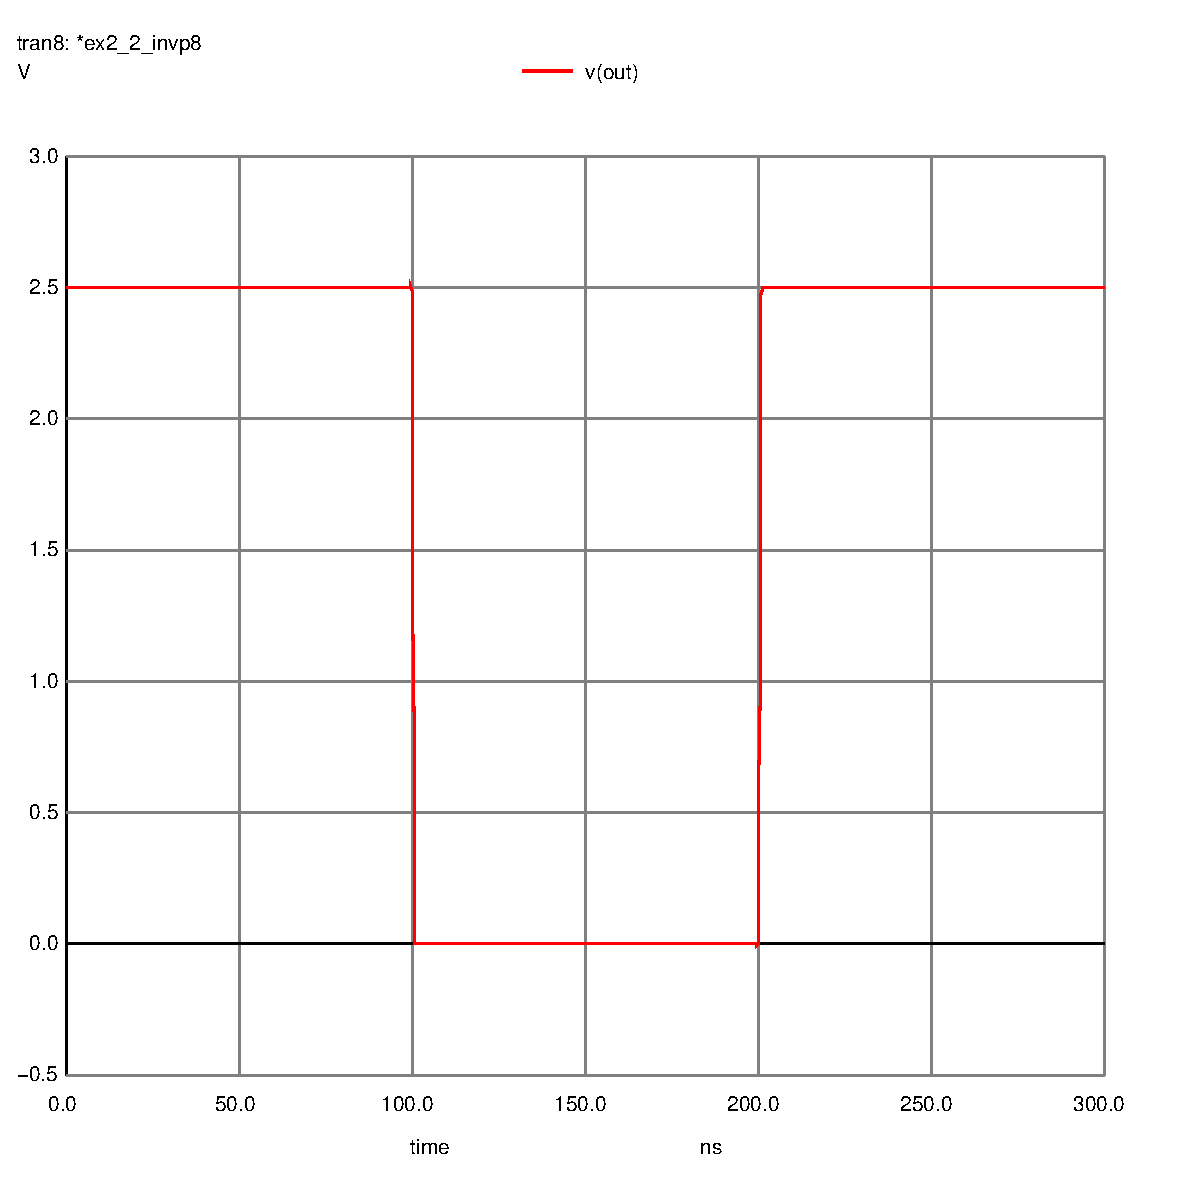
\includegraphics[scale=0.8]{ex2_2_invp8.ps}
    \vspace{30pt}
    \caption{サイズ8倍のインバータを負荷として接続}
\end{figure}

\subsubsection{負荷が2入力NAND回路の場合}
\begin{figure}[H]
    \centering
    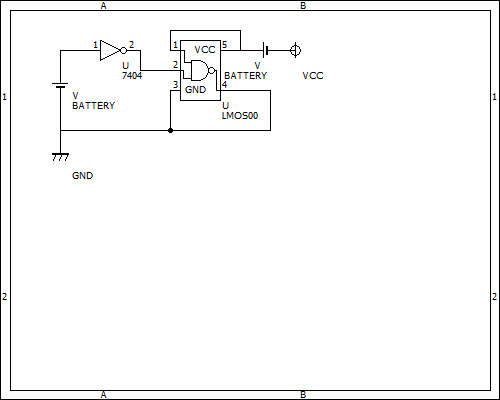
\includegraphics[bb=0 0 500 400]{ex2_2_nand.png}
    \caption{NAND回路を負荷とした時の回路図}
\end{figure}

\begin{flushleft}
    立ち上がり: $5.86 \cdot ^{-11}$\\
    立ち下り: $1.991 \cdot 10^{-10}$
\end{flushleft}
\begin{figure}[H]
    \hspace{50pt}
    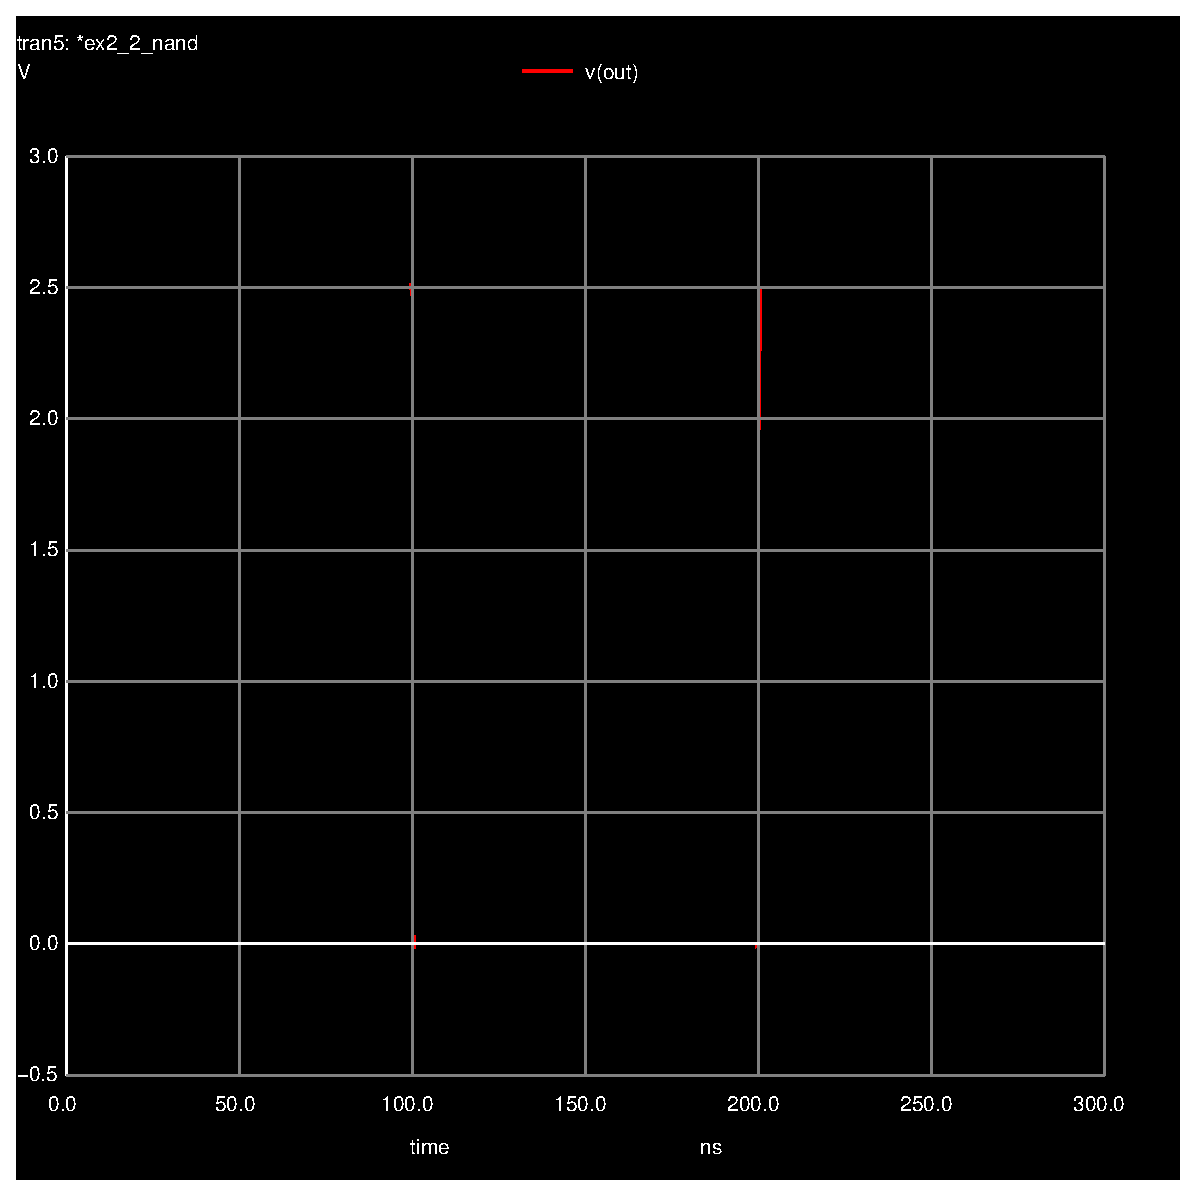
\includegraphics[scale=0.8]{ex2_2_nand.ps}
    \vspace{30pt}
    \caption{NAND回路を負荷として接続}
\end{figure}


\subsection{比較}
\begin{table}[H]
    \caption{ファンアウトでの比較}
    \centering
    \begin{tabular}{|l|c|c|c|} \hline
        &負荷がインバータ&負荷が2つのインバータ&負荷が3つのインバータ \\ \hline \hline
        立ち上がり($10^{-11} s$)&3.86&8.04&11.68\\
        立下り($10^{-11} s$)&18.46&22.49&26.73\\
        \hline
    \end{tabular}
\end{table}

\begin{table}[H]
    \caption{サイズでの比較}
    \centering
    \begin{tabular}{|l|c|c|c|c|} \hline
        &負荷がインバータ&負荷がサイズ2倍&負荷がサイズ4倍&負荷がサイズ8倍\\ \hline \hline
        立ち上がり($10^{-11} s$)&3.86&8.01&15.25&25.93\\
        立下り($10^{-11} s$)&18.46&22.43&29.64&40.24\\
        \hline
    \end{tabular}
\end{table}

\begin{table}[H]
    \caption{違う論理素子での比較}
    \centering
    \begin{tabular}{|l|c|c|} \hline
        &負荷がインバータ&負荷がNAND回路\\ \hline \hline
        立ち上がり($10^{-11} s$)&3.86&5.86\\ 
        立下り($10^{-11} s$)&18.46&19.91\\
        \hline
    \end{tabular}
\end{table}

\subsection{考察}
得られた結果を観察すると、ファンアウトやサイズが数倍になるとそれらが小さいときは立ち上がりは線型的に変化しているが大きくなると変化がゆるやかになっている。立下りについては逆のことが言える。
文献調査をした結果得られた情報によると、インバータの遅延時間には負荷容量依存性とチャネル幅依存性があることが分かった。負荷容量が大きいと遅延時間は長く、チャネル幅が大きいと遅延時間は短くなることが分かった。今回の実験では測定するインバータのチャネル幅は変えないため、負荷容量について考える。遅延時間は$C$を負荷容量、$I$をインバータの駆動電流として$t_{r} \simeq \frac{C \cdot Vdd}{I}$と表される。これは遅延時間は近似として、コンデンサの充電/放電に要する時間と見れるからである。回路の構成を変えると上記の式のうちで負荷容量が変化していく。
また負荷容量には動作モード依存性があることも分かった。
具体的には飽和領域では$C$は小さいが、線型領域では$C$は大きい。
つまり同じ構成でも$C$の値が変わっていくので上の式を少し修正して$\int_0^{t_{r}} I \cdot dt = \int_0^{t_{r}} Vdd \cdot \frac{C(t)}{dt} \cdot dt$ とする。
$C(t_r)$の変化は
\begin{url}
    {http://www.ssc.pe.titech.ac.jp/lectures/icTitech/091014_Titech_IC_03.pdf}
\end{url}の21枚目のスライドを参照されたい。
入力が立ち上がりの時は線型領域$\rightarrow$飽和領域となり、立下りの時には飽和領域$\rightarrow$線型領域となるので、ファンアウトやサイズが大きくなると$C(t_r)$は大きくなり遅延時間もおおきくなるが、上式において$t_r$が大きくなると立ち上がりでは線型領域から飽和領域に突入し$\frac{dC(t)}{dt}$は小さくなるので増加は徐々に線型的でなくなっていく。
逆に立下りでは、最初は飽和領域から始まるのでサイズが大きくなるにつれて線型的になっていくといえる。
これは測定した結果と一致していると思う。
上では違う論理素子での比較もしたが、上に述べたような理由で立ち上がりに関しては遅延時間の差が目立つが、立下りでは遅延時間の差は比較的小さい。


\section{課題3}


\subsection{4入力NANDとNOTでの構成}
\subsubsection{手順}
配布された資料通りの回路を記述し、その記述ファイル内でmeasコマンドを駆使して出力が$1.25V$となる点を8つ求めた。入力が$1.25V$となる時刻は自分で書いた回路記述ファイルからわかるのでmeasコマンドで求めることはしなかった。
以下に回路図を示す。
\begin{figure}[H]
    \centering
    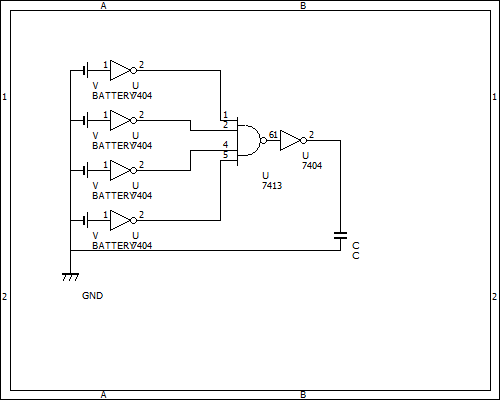
\includegraphics[bb=0 0 500 400]{ex3_nand_not.png}
    \caption{4入力NANDとNOTを用いた回路図}
\end{figure}

\subsubsection{結果}
\begin{flushleft}
$(1,1,1,1) \rightarrow (1,1,1,0) : 8.7701 \cdot 10^{-10}$\\
$(1,1,1,0) \rightarrow (1,1,1,1) : 1.0673 \cdot 10^{-9}$\\
$(1,1,1,1) \rightarrow (1,1,0,1) : 9.15 \cdot 10^{-10}$\\
$(1,1,0,1) \rightarrow (1,1,1,1) : 1.0839 \cdot 10^{-9}$\\
$(1,1,1,1) \rightarrow (1,0,1,1) : 9.497 \cdot 10^{-10}$\\
$(1,0,1,1) \rightarrow (1,1,1,1) : 1.0948 \cdot 10^{-9}$\\
$(1,1,1,1) \rightarrow (0,1,1,1) : 9.857 \cdot 10^{-10}$\\
$(0,1,1,1) \rightarrow (1,1,1,1) : 1.1089 \cdot 10^{-9}$\\
average: $10.10289 \cdot 10^{-10}$

\end{flushleft}
\begin{figure}[H]
    \hspace{50pt}
    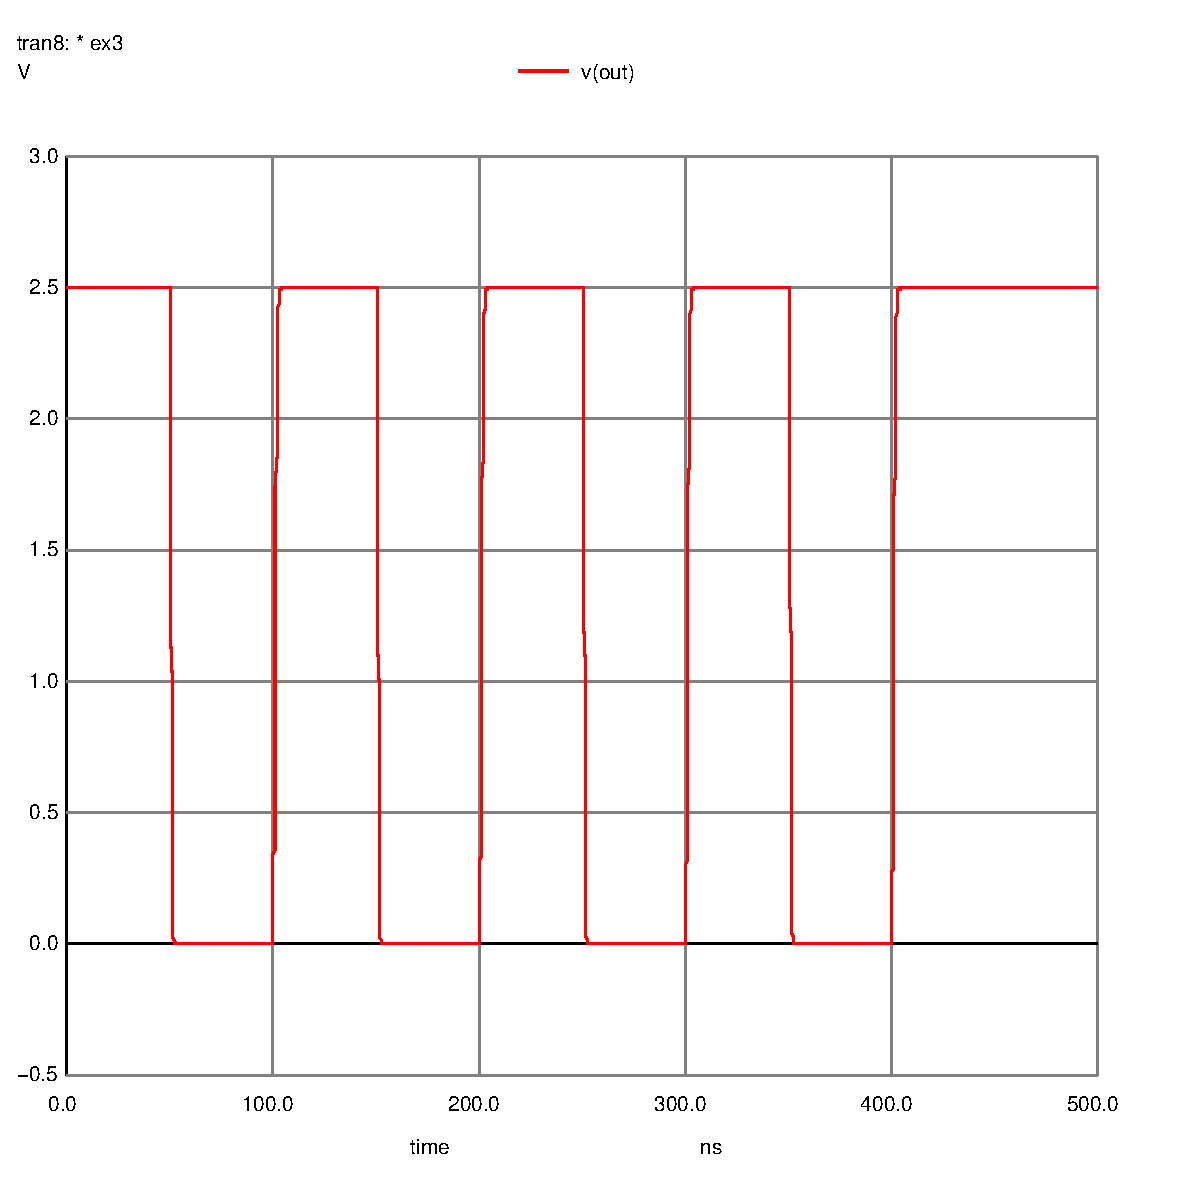
\includegraphics[scale=0.8]{ex3.ps}
    \vspace{30pt}
    \caption{4入力NANDとNOT回路による構成}
\end{figure}



\subsection{2入力NANDと2入力NORでの構成}
\subsubsection{手順}
上と同様に資料にある図を記述し、コマンドを使って出力が$1.25V$を指す点の時刻を測定した。
以下に回路図を示す。
\begin{figure}[H]
    \centering
    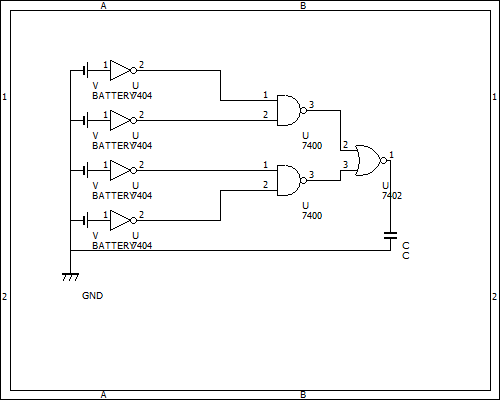
\includegraphics[bb=0 0 500 400]{ex3_nand_nand_nor.png}
    \caption{2入力NANDと2入力NORを用いた回路図}
\end{figure}

\subsubsection{結果}
\begin{flushleft}
    $(1,1,1,1) \rightarrow (1,1,1,0) : 8.3815 \cdot 10^{-10}$\\
    $(1,1,1,0) \rightarrow (1,1,1,1) : 9.555 \cdot 10^{-10}$\\
    $(1,1,1,1) \rightarrow (1,1,0,1) : 8.619 \cdot 10^{-10}$\\
    $(1,1,0,1) \rightarrow (1,1,1,1) : 9.606 \cdot 10^{-10}$\\
    $(1,1,1,1) \rightarrow (1,0,1,1) : 8.6 \cdot 10^{-10}$\\
    $(1,0,1,1) \rightarrow (1,1,1,1) : 9.74 \cdot 10^{-10}$\\
    $(1,1,1,1) \rightarrow (0,1,1,1) : 8.764 \cdot 10^{-10}$\\
    $(0,1,1,1) \rightarrow (1,1,1,1) : 9.801 \cdot 10^{-10}$\\
    average: $9.801 \cdot 10^{-10}$
    
    \end{flushleft}
    \begin{figure}[H]
        \hspace{50pt}
        \includegraphics[scale=0.8]{ex3_2.ps}
        \vspace{30pt}
        \caption{2入力NANDと2入力NANDによる構成}
    \end{figure}

\subsection{サイズ2倍の4入力NANDとNOT回路での構成}
\subsubsection{手順}
    同上のため省略。
    以下に回路図を示す。
    \begin{figure}[H]
        \centering
        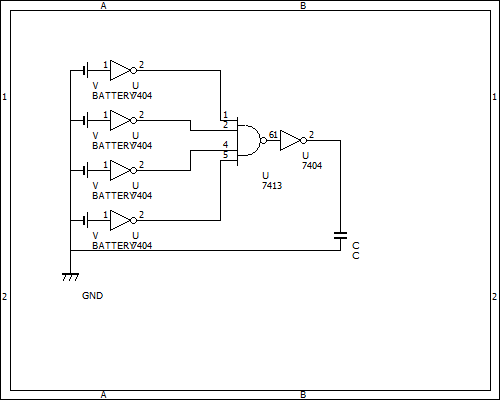
\includegraphics[bb=0 0 500 400]{ex3_nand_not.png}
        \caption{サイズ2倍の4入力NANDとNOTを用いた回路図}
    \end{figure}
\subsubsection{結果}
\begin{flushleft}
    $(1,1,1,1) \rightarrow (1,1,1,0) : 9.5186 \cdot 10^{-10}$\\
    $(1,1,1,0) \rightarrow (1,1,1,1) : 11.256 \cdot 10^{-10}$\\
    $(1,1,1,1) \rightarrow (1,1,0,1) : 9.857 \cdot 10^{-10}$\\
    $(1,1,0,1) \rightarrow (1,1,1,1) : 11.423 \cdot 10^{-10}$\\
    $(1,1,1,1) \rightarrow (1,0,1,1) : 10.227 \cdot 10^{-10}$\\
    $(1,0,1,1) \rightarrow (1,1,1,1) : 11.547 \cdot 10^{-10}$\\
    $(1,1,1,1) \rightarrow (0,1,1,1) : 10.676 \cdot 10^{-10}$\\
    $(0,1,1,1) \rightarrow (1,1,1,1) : 11.676 \cdot 10^{-10}$\\
    average: $10.77257 \cdot 10^{-10}$
    
    \end{flushleft}
    \begin{figure}[H]
        \hspace{50pt}
        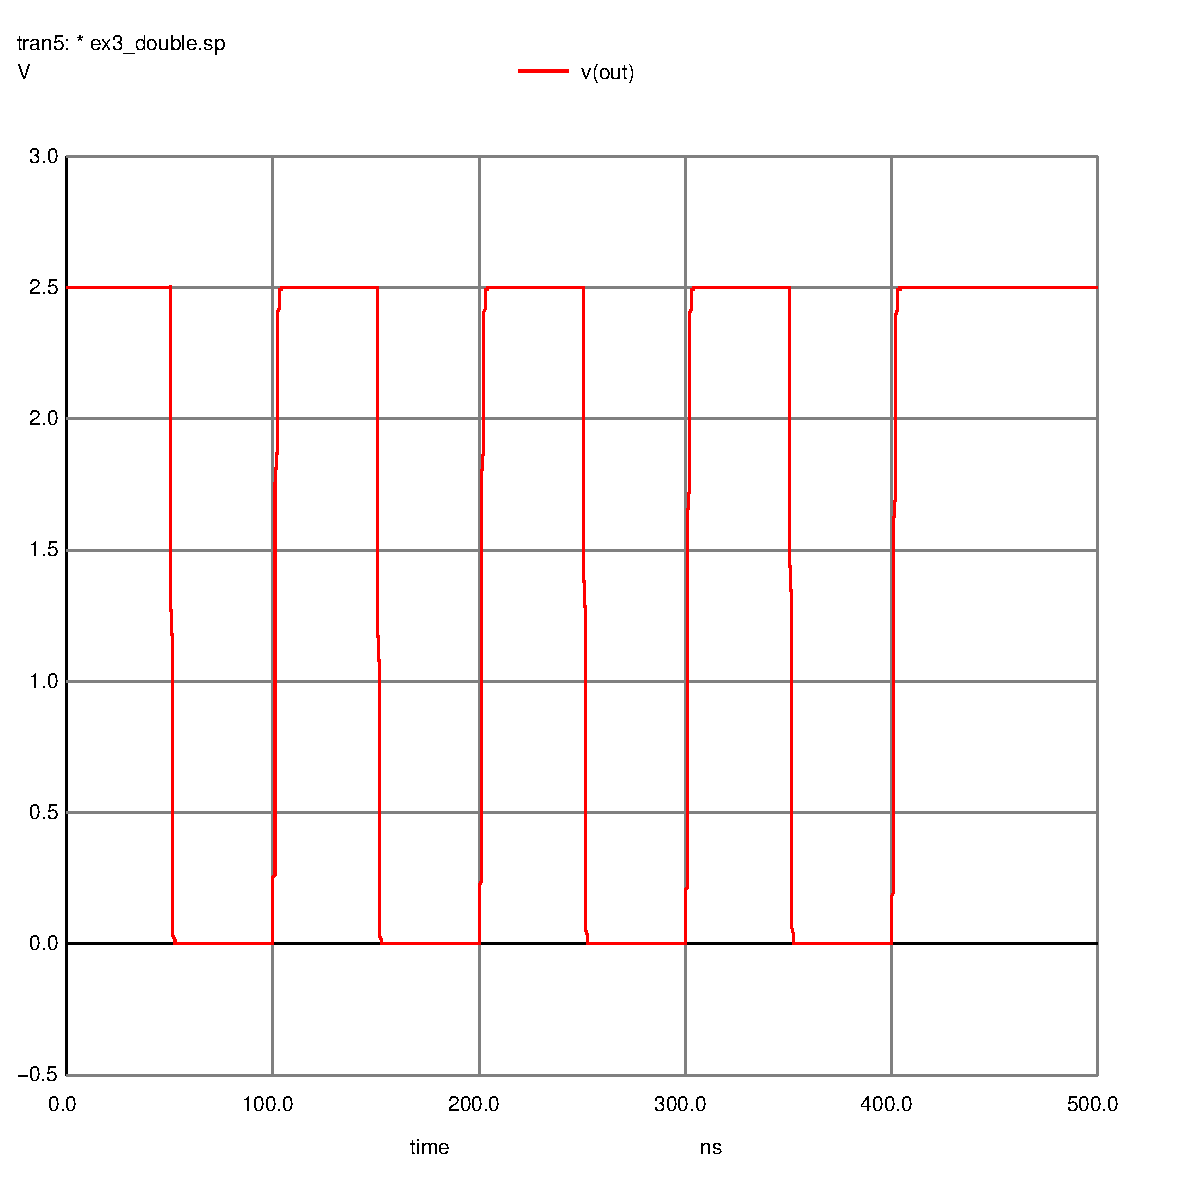
\includegraphics[scale=0.8]{ex3_double.ps}
        \vspace{30pt}
        \caption{サイズ2倍の4入力NANDとNOT回路による構成}
    \end{figure}

\subsection{4入力NANDとサイズ2倍のNOT回路による構成}
\subsubsection{手順}
    同上のため省略。
    以下に回路図を示す。
    \begin{figure}[H]
        \centering
        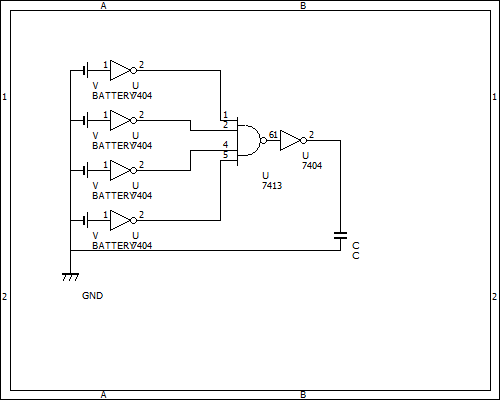
\includegraphics[bb=0 0 500 400]{ex3_nand_not.png}
        \caption{4入力NANDとサイズ2倍のNOTを用いた回路図}
    \end{figure}
\subsubsection{結果}
\begin{flushleft}
$(1,1,1,1) \rightarrow (1,1,1,0) : 7.4875 \cdot 10^{-10}$\\
$(1,1,1,0) \rightarrow (1,1,1,1) : 5.85 \cdot 10^{-10}$\\
$(1,1,1,1) \rightarrow (1,1,0,1) : 7.731 \cdot 10^{-10}$\\
$(1,1,0,1) \rightarrow (1,1,1,1) : 6.067 \cdot 10^{-10}$\\
$(1,1,1,1) \rightarrow (1,0,1,1) : 7.954 \cdot 10^{-10}$\\
$(1,0,1,1) \rightarrow (1,1,1,1) : 6.202 \cdot 10^{-10}$\\
$(1,1,1,1) \rightarrow (0,1,1,1) : 8.179 \cdot 10^{-10}$\\
$(0,1,1,1) \rightarrow (1,1,1,1) : 6.29 \cdot 10^{-10}$\\
average: $6.970062 \cdot 10^{-10}$

\end{flushleft}
\begin{figure}[H]
    \hspace{50pt}
    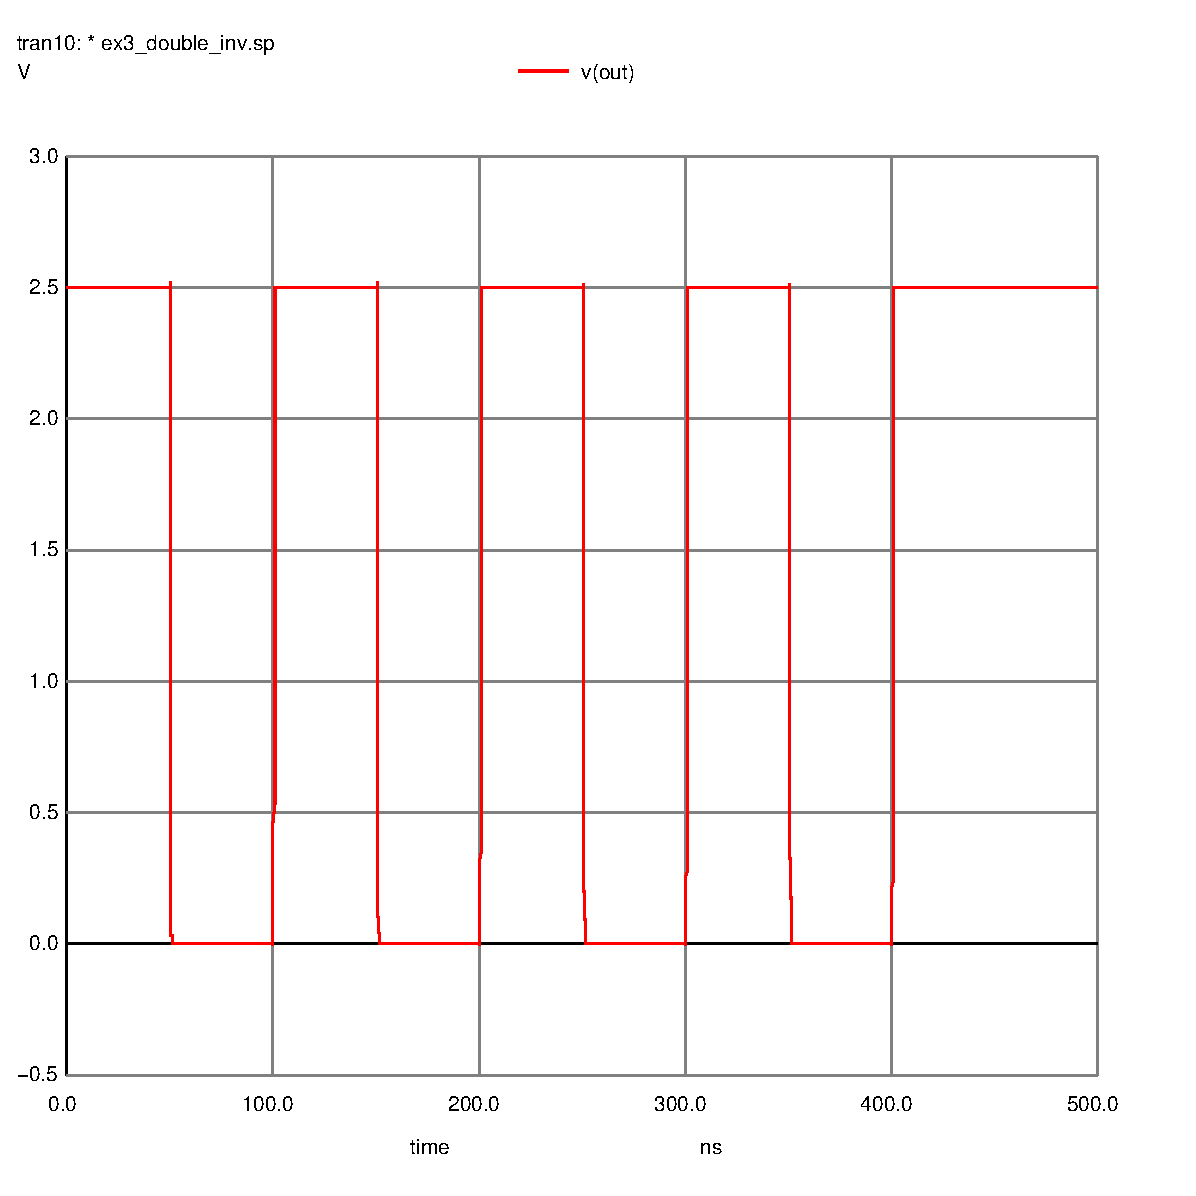
\includegraphics[scale=0.8]{ex3_double_inv.ps}
    \vspace{30pt}
    \caption{4入力NANDとサイズ2倍のNOT回路による構成}
\end{figure}

\subsection{2入力NANDとサイズ2倍のNOR回路による構成}
\subsubsection{手順}
    同上のため省略。
    以下に回路図を示す。
    \begin{figure}[H]
        \centering
        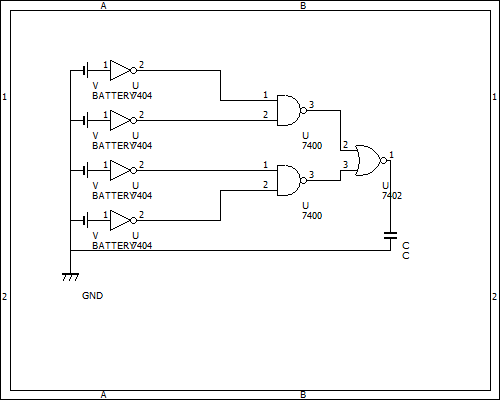
\includegraphics[bb=0 0 500 400]{ex3_nand_nand_nor.png}
        \caption{2入力NANDとサイズ2倍の2入力NORを用いた回路図}
    \end{figure}
\subsubsection{結果}
\begin{flushleft}
$(1,1,1,1) \rightarrow (1,1,1,0) : 5.986 \cdot 10^{-10}$\\
$(1,1,1,0) \rightarrow (1,1,1,1) : 6.803 \cdot 10^{-10}$\\
$(1,1,1,1) \rightarrow (1,1,0,1) : 6.197 \cdot 10^{-10}$\\
$(1,1,0,1) \rightarrow (1,1,1,1) : 6.874 \cdot 10^{-10}$\\
$(1,1,1,1) \rightarrow (1,0,1,1) : 6.127 \cdot 10^{-10}$\\
$(1,0,1,1) \rightarrow (1,1,1,1) : 7.066 \cdot 10^{-10}$\\
$(1,1,1,1) \rightarrow (0,1,1,1) : 6.364 \cdot 10^{-10}$\\
$(0,1,1,1) \rightarrow (1,1,1,1) : 7.102 \cdot 10^{-10}$\\
average: $6.564875 \cdot 10^{-10}$

\end{flushleft}
\begin{figure}[H]
    \hspace{50pt}
    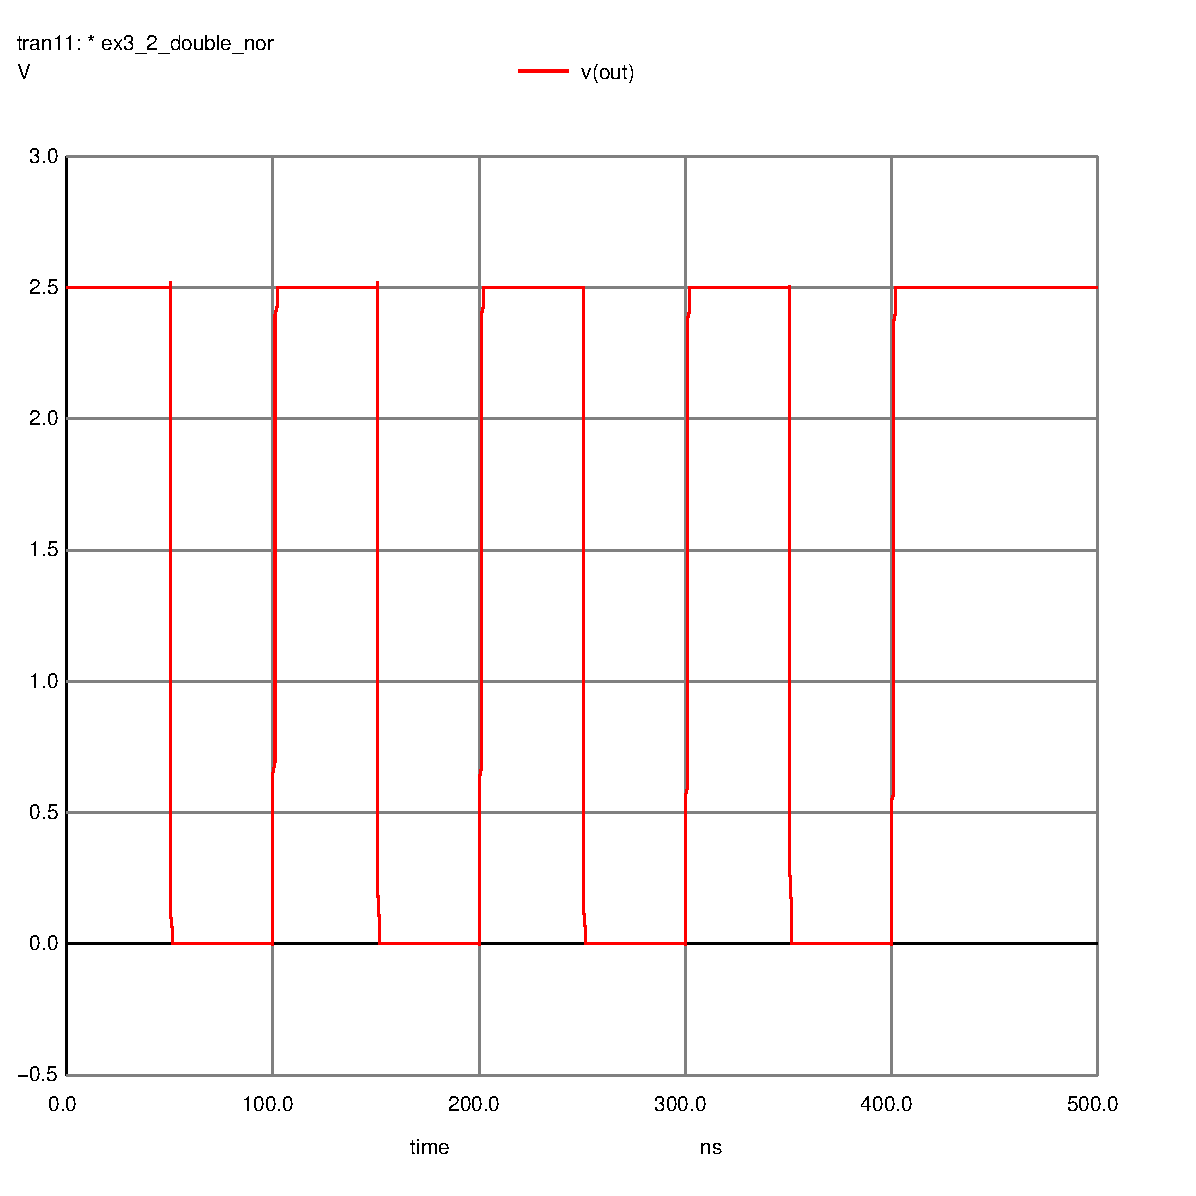
\includegraphics[scale=0.8]{ex3_2_double_nor.ps}
    \vspace{30pt}
    \caption{2入力NANDとサイズ2倍のNOR回路による構成}
\end{figure}

\subsection{比較}
遅延時間の基準として各々の遅延時間の平均を採用した。
\begin{table}[H]
    \caption{遅延時間の比較}
    \centering
    \begin{tabular}{|l|c|c|c|c|c|}\hline
        &nand4-inv&nand4p2-inv&nand4-invp2&nand2-nor&nand2-norp2\\ \hline
        latency($10^{-10}$)&10.10289&10.77257&6.970062&9.801&6.564875\\ \hline
    \end{tabular}
\end{table}

\subsection{考察}
得られた結果からわかることとして、後段の論理素子のサイズを大きくすると遅延時間が改善していることがわかる。
さらに、一つの素子に入力を集中させるよりも分散させて入力したほうがわずかに遅延時間が短いことがわかる。
論理素子のサイズが変わることでその素子の容量が変わるので、容量が遅延時間に影響していると思われる。このことから後段の容量を大きくして、入力のサイズが小さな素子を用いて回路を構成すればよいと思わる。

\section{コード}
\begin{lstlisting}
    * ex1_dif.sp
.options post temp=27

v1 in 0 pwl ( 0.0u 0.0
+	      99.5u 0.0
+	      100.5u 2.5
+	      199.5u 2.5
+	      200.5u 0.0 )
c1 in out 510.0p 
r1 out 0 10.0k 


.tran 0.1u 300u
.control
set hcopydevtype=postscript
set hcopypscolor=1
set color0=rgb:0/0/0
run
hardcopy ex1_dif.ps v(out)
meas tran vMax FIND v(out) WHEN time=100.5u
let vMid=vMax*0.37
*teval2 is a half amp time of output
meas tran teval2 WHEN v(out)=vMid CROSS=2
*100.0u is a half amp time of input
let delta=teval2-100.0u
print delta
.endc

.end
\end{lstlisting}

\begin{lstlisting}
    * ex1_integral.sp
    .options post temp=27
    
    v1 in 0 pwl ( 0.0u 0.0
    +	      99.5u 0.0
    +	      100.5u 2.5
    +	      199.5u 2.5
    +	      200.5u 0.0 )
    c1 out 0 510.0p 
    r1 in out 10.0k 
    
    
    .tran 0.1u 300u
    
    .control
    set hcopydevtype=postscript
    set hcopypscolor=1
    set color0=rgb:0/0/0
    run
    hardcopy ex1_integral.ps v(out)
    *vMid is 63% of the amp
    let vMid=2.5*0.63
    *teval2 is the time when v indicate vMid
    meas tran teval2 WHEN v(out)=vMid
    let delta=teval2-100.0u
    print delta
    .endc
    
    .end
    
\end{lstlisting}

\begin{lstlisting}
    * ex2_1
    .options post temp=27
    .include mos_model3
    .include logic.cir
    
    
    v1 in 0 pwl ( 0.0n 0.0
    +	      99.5n 0.0
    +	      100.5n 2.5
    +	      199.5n 2.5
    +	      200.5n 0.0 )
    X1 in out Vdd inv
    v2 Vdd 0 2.5v
    c1 out 0 30f
    
    
    
    .tran 0.1n 300n
    
    .control
    set hcopydevtype=postscript
    set hcopypscolor=1
    set color0=rgb:0/0/0
    run
    hardcopy ex2_1.ps v(out)
    meas tran teval1 WHEN v(out)=1.25 CROSS=1
    let delta1=teval1-100n
    print delta1
    meas tran teval2 WHEN v(out)=1.25 CROSS=2
    let delta2=teval2-200n
    print delta2
    .endc
    
    .end
    
\end{lstlisting}

\begin{lstlisting}
    *ex2_2_double_inv
    .options post temp=27
    .include mos_model3
    .include logic.cir
    
    
    v1 in 0 pwl ( 0.0n 0.0
    +	      99.5n 0.0
    +	      100.5n 2.5
    +	      199.5n 2.5
    +	      200.5n 0.0 )
    X1 in out Vdd inv
    X2 out 0 Vdd inv
    X3 out 0 Vdd inv
    v2 Vdd 0 2.5v
    
    
    .tran 0.1n 300n
    
    .control
    set hcopydevtype=postscript
    set hcopypscolor=1
    set color0=rgb:0/0/0
    run
    hardcopy ex2_2_double_inv.ps v(out)
    meas tran teval1 WHEN v(out)=1.25 CROSS=1
    let delta1=teval1-100n
    print delta1
    meas tran teval2 WHEN v(out)=1.25 CROSS=2
    let delta2=teval2-200n
    print delta2
    .endc
    
    .end
\end{lstlisting}

\begin{lstlisting}
    *ex2_2_triple_inv
    .options post temp=27
    .include mos_model3
    .include logic.cir
    
    
    v1 in 0 pwl ( 0.0n 0.0
    +	      99.5n 0.0
    +	      100.5n 2.5
    +	      199.5n 2.5
    +	      200.5n 0.0 )
    X1 in out Vdd inv
    X2 out 0 Vdd inv
    X3 out 0 Vdd inv
    X4 out 0 Vdd inv
    v2 Vdd 0 2.5v
    
    
    .tran 0.1n 300n
    
    .control
    set hcopydevtype=postscript
    set hcopypscolor=1
    set color0=rgb:0/0/0
    run
    hardcopy ex2_2_triple_inv.ps v(out)
    meas tran teval1 WHEN v(out)=1.25 CROSS=1
    let delta1=teval1-100n
    print delta1
    meas tran teval2 WHEN v(out)=1.25 CROSS=2
    let delta2=teval2-200n
    print delta2
    .endc
    
    .end
\end{lstlisting}

\begin{lstlisting}
    *ex2_2_invp2
    .options post temp=27
    .include mos_model3
    .include logic.cir
    
    
    v1 in 0 pwl ( 0.0n 0.0
    +	      99.5n 0.0
    +	      100.5n 2.5
    +	      199.5n 2.5
    +	      200.5n 0.0 )
    X1 in out Vdd inv
    X2 out 0 Vdd invp2
    v2 Vdd 0 2.5v
    
    
    .tran 0.1n 300n
    
    .control
    set hcopydevtype=postscript
    set hcopypscolor=1
    set color0=rgb:0/0/0
    run
    hardcopy ex2_2_invp2.ps v(out)
    meas tran teval1 WHEN v(out)=1.25 CROSS=1
    let delta1=teval1-100n
    print delta1
    meas tran teval2 WHEN v(out)=1.25 CROSS=2
    let delta2=teval2-200n
    print delta2
    .endc
    
    .end
\end{lstlisting}

\begin{lstlisting}
    *ex2_2_invp4
    .options post temp=27
    .include mos_model3
    .include logic.cir
    
    
    v1 in 0 pwl ( 0.0n 0.0
    +	      99.5n 0.0
    +	      100.5n 2.5
    +	      199.5n 2.5
    +	      200.5n 0.0 )
    X1 in out Vdd inv
    X4 out 0 Vdd invp4
    v2 Vdd 0 2.5v
    
    
    .tran 0.1n 300n
    
    .control
    set hcopydevtype=postscript
    set hcopypscolor=1
    set color0=rgb:0/0/0
    run
    hardcopy ex2_2_invp4.ps v(out)
    meas tran teval1 WHEN v(out)=1.25 CROSS=1
    let delta1=teval1-100n
    print delta1
    meas tran teval2 WHEN v(out)=1.25 CROSS=2
    let delta2=teval2-200n
    print delta2
    .endc
    
    .end
\end{lstlisting}

\begin{lstlisting}
    *ex2_2_invp8
    .options post temp=27
    .include mos_model3
    .include logic.cir
    
    
    v1 in 0 pwl ( 0.0n 0.0
    +	      99.5n 0.0
    +	      100.5n 2.5
    +	      199.5n 2.5
    +	      200.5n 0.0 )
    X1 in out Vdd inv
    X2 out 0 Vdd invp8
    v2 Vdd 0 2.5v
    
    
    .tran 0.1n 300n
    
    .control
    set hcopydevtype=postscript
    set hcopypscolor=1
    set color0=rgb:0/0/0
    run
    hardcopy ex2_2_invp8.ps v(out)
    meas tran teval1 WHEN v(out)=1.25 CROSS=1
    let delta1=teval1-100n
    print delta1
    meas tran teval2 WHEN v(out)=1.25 CROSS=2
    let delta2=teval2-200n
    print delta2
    .endc
    
    .end
\end{lstlisting}

\begin{lstlisting}
    *ex2_2_nand
    .options post temp=27
    .include mos_model3
    .include logic.cir
    
    
    v1 in 0 pwl ( 0.0n 0.0
    +	      99.5n 0.0
    +	      100.5n 2.5
    +	      199.5n 2.5
    +	      200.5n 0.0 )
    X1 in out Vdd inv
    X2 Vdd out 0 Vdd nand2
    v2 Vdd 0 2.5v
    
    
    .tran 0.1n 300n
    
    .control
    set hcopydevtype=postscript
    set hcopypscolor=1
    set color0=rgb:0/0/0
    run
    hardcopy ex2_2_nand.ps v(out)
    meas tran teval1 WHEN v(out)=1.25 CROSS=1
    let delta1=teval1-100n
    print delta1
    meas tran teval2 WHEN v(out)=1.25 CROSS=2
    let delta2=teval2-200n
    print delta2
    .endc
    
    .end
\end{lstlisting}

\begin{lstlisting}

\end{lstlisting}

\begin{lstlisting}
    * ex3
    .options post temp=27
    .include mos_model3
    .include logic.cir
    
    
    v1 in1 0 pwl ( 0.0n 0.0 49.5n 0.0 50.5n 2.5 99.5n 2.5 100.5n 0.0 )
    
    v2 in2 0 pwl ( 0.0n 0.0 149.5n 0.0 150.5n 2.5 199.5n 2.5 200.5n 0.0 )
    
    v3 in3 0 pwl ( 0.0n 0.0 249.5n 0.0 250.5n 2.5 299.5n 2.5 300.5n 0.0 )
    
    v4 in4 0 pwl ( 0.0n 0.0 349.5n 0.0 350.5n 2.5 399.5n 2.5 400.5n 0.0 )
    
    vc Vdd 0 2.5v
    
    
    X1 in1 in1_and Vdd inv
    X2 in2 in2_and Vdd inv
    X3 in3 in3_and Vdd inv
    X4 in4 in4_and Vdd inv
    X5 in1_and in2_and in3_and in4_and out_nand Vdd nand4
    X6 out_nand out Vdd inv
    c1 out 0 500f
    
    .tran 0.1n 500n
    
    .control
    set hcopydevtype=postscript
    set hcopypscolor=1
    set color0=rgb:0/0/0
    run
    hardcopy ex3.ps v(out)
    meas tran teval1 WHEN v(out)=1.25 CROSS=1
    meas tran teval2 WHEN v(out)=1.25 CROSS=2
    meas tran teval3 WHEN v(out)=1.25 CROSS=3
    meas tran teval4 WHEN v(out)=1.25 CROSS=4
    meas tran teval5 WHEN v(out)=1.25 CROSS=5
    meas tran teval6 WHEN v(out)=1.25 CROSS=6
    meas tran teval7 WHEN v(out)=1.25 CROSS=7
    meas tran teval8 WHEN v(out)=1.25 CROSS=8
    let delta1=teval1-50.0n
    print delta1
    let delta2=teval2-100.0n
    print delta2
    let delta3=teval3-150.0n
    print delta3
    let delta4=teval4-200.0n
    print delta4
    let delta5=teval5-250.0n
    print delta5
    let delta6=teval6-300.0n
    print delta6
    let delta7=teval7-350.0n
    print delta7
    let delta8=teval8-400.0n
    print delta8
    let average=(delta1+delta2+delta3
    + +delta4+delta5+delta6+delta7+delta8)/8
    print average
    .endc
    
    .end
    
\end{lstlisting}

\begin{lstlisting}
    * ex3_2
    .options post temp=27
    .include mos_model3
    .include logic.cir
    
    
    v1 in1 0 pwl ( 0.0n 0.0 49.5n 0.0 50.5n 2.5 99.5n 2.5 100.5n 0.0 )
    
    v2 in2 0 pwl ( 0.0n 0.0 149.5n 0.0 150.5n 2.5 199.5n 2.5 200.5n 0.0 )
    
    v3 in3 0 pwl ( 0.0n 0.0 249.5n 0.0 250.5n 2.5 299.5n 2.5 300.5n 0.0 )
    
    v4 in4 0 pwl ( 0.0n 0.0 349.5n 0.0 350.5n 2.5 399.5n 2.5 400.5n 0.0 )
    
    vc Vdd 0 2.5v
    
    
    X1 in1 in1_and Vdd inv
    X2 in2 in2_and Vdd inv
    X3 in3 in3_and Vdd inv
    X4 in4 in4_and Vdd inv
    X5 in1_and in2_and out_nand1 Vdd nand2
    X6 in3_and in4_and out_nand2 Vdd nand2
    X7 out_nand1 out_nand2 out Vdd nor2
    c1 out 0 500f
    
    .tran 0.1n 500n
    
    .control
    set hcopydevtype=postscript
    set hcopypscolor=1
    set color0=rgb:0/0/0
    run
    hardcopy ex3_2.ps v(out)
    meas tran teval1 WHEN v(out)=1.25 CROSS=1
    meas tran teval2 WHEN v(out)=1.25 CROSS=2
    meas tran teval3 WHEN v(out)=1.25 CROSS=3
    meas tran teval4 WHEN v(out)=1.25 CROSS=4
    meas tran teval5 WHEN v(out)=1.25 CROSS=5
    meas tran teval6 WHEN v(out)=1.25 CROSS=6
    meas tran teval7 WHEN v(out)=1.25 CROSS=7
    meas tran teval8 WHEN v(out)=1.25 CROSS=8
    let delta1=teval1-50.0n
    print delta1
    let delta2=teval2-100.0n
    print delta2
    let delta3=teval3-150.0n
    print delta3
    let delta4=teval4-200.0n
    print delta4
    let delta5=teval5-250.0n
    print delta5
    let delta6=teval6-300.0n
    print delta6
    let delta7=teval7-350.0n
    print delta7
    let delta8=teval8-400.0n
    print delta8
    let average=(delta1+delta2+delta3
    + +delta4+delta5+delta6+delta7+delta8)/8
    print average
    .endc
    
    .end
\end{lstlisting}

\begin{lstlisting}
    * ex3_double_nand.sp
    .options post temp=27
    .include mos_model3
    .include logic.cir
    
    
    v1 in1 0 pwl ( 0.0n 0.0 49.5n 0.0 50.5n 2.5 99.5n 2.5 100.5n 0.0 )
    
    v2 in2 0 pwl ( 0.0n 0.0 149.5n 0.0 150.5n 2.5 199.5n 2.5 200.5n 0.0 )
    
    v3 in3 0 pwl ( 0.0n 0.0 249.5n 0.0 250.5n 2.5 299.5n 2.5 300.5n 0.0 )
    
    v4 in4 0 pwl ( 0.0n 0.0 349.5n 0.0 350.5n 2.5 399.5n 2.5 400.5n 0.0 )
    
    vc Vdd 0 2.5v
    
    
    X1 in1 in1_and Vdd inv
    X2 in2 in2_and Vdd inv
    X3 in3 in3_and Vdd inv
    X4 in4 in4_and Vdd inv
    X5 in1_and in2_and in3_and in4_and out_nand Vdd nand4p2
    X6 out_nand out Vdd inv
    c1 out 0 500f
    
    .tran 0.1n 500n
    
    .control
    set hcopydevtype=postscript
    set hcopypscolor=1
    set color0=rgb:0/0/0
    run
    hardcopy ex3_double_nand.ps v(out)
    meas tran teval1 WHEN v(out)=1.25 CROSS=1
    meas tran teval2 WHEN v(out)=1.25 CROSS=2
    meas tran teval3 WHEN v(out)=1.25 CROSS=3
    meas tran teval4 WHEN v(out)=1.25 CROSS=4
    meas tran teval5 WHEN v(out)=1.25 CROSS=5
    meas tran teval6 WHEN v(out)=1.25 CROSS=6
    meas tran teval7 WHEN v(out)=1.25 CROSS=7
    meas tran teval8 WHEN v(out)=1.25 CROSS=8
    let delta1=teval1-50.0n
    print delta1
    let delta2=teval2-100.0n
    print delta2
    let delta3=teval3-150.0n
    print delta3
    let delta4=teval4-200.0n
    print delta4
    let delta5=teval5-250.0n
    print delta5
    let delta6=teval6-300.0n
    print delta6
    let delta7=teval7-350.0n
    print delta7
    let delta8=teval8-400.0n
    print delta8
    let average=(delta1+delta2+delta3
    + +delta4+delta5+delta6+delta7+delta8)/8
    print average
    .endc
    
    .end
    
\end{lstlisting}

\begin{lstlisting}
    * ex3_double_inv.sp
    .options post temp=27
    .include mos_model3
    .include logic.cir
    
    
    v1 in1 0 pwl ( 0.0n 0.0 49.5n 0.0 50.5n 2.5 99.5n 2.5 100.5n 0.0 )
    
    v2 in2 0 pwl ( 0.0n 0.0 149.5n 0.0 150.5n 2.5 199.5n 2.5 200.5n 0.0 )
    
    v3 in3 0 pwl ( 0.0n 0.0 249.5n 0.0 250.5n 2.5 299.5n 2.5 300.5n 0.0 )
    
    v4 in4 0 pwl ( 0.0n 0.0 349.5n 0.0 350.5n 2.5 399.5n 2.5 400.5n 0.0 )
    
    vc Vdd 0 2.5v
    
    
    X1 in1 in1_and Vdd inv
    X2 in2 in2_and Vdd inv
    X3 in3 in3_and Vdd inv
    X4 in4 in4_and Vdd inv
    X5 in1_and in2_and in3_and in4_and out_nand Vdd nand4
    X6 out_nand out Vdd invp2
    c1 out 0 500f
    
    .tran 0.1n 500n
    
    .control
    set hcopydevtype=postscript
    set hcopypscolor=1
    set color0=rgb:0/0/0
    run
    hardcopy ex3_double_inv.ps v(out)
    meas tran teval1 WHEN v(out)=1.25 CROSS=1
    meas tran teval2 WHEN v(out)=1.25 CROSS=2
    meas tran teval3 WHEN v(out)=1.25 CROSS=3
    meas tran teval4 WHEN v(out)=1.25 CROSS=4
    meas tran teval5 WHEN v(out)=1.25 CROSS=5
    meas tran teval6 WHEN v(out)=1.25 CROSS=6
    meas tran teval7 WHEN v(out)=1.25 CROSS=7
    meas tran teval8 WHEN v(out)=1.25 CROSS=8
    let delta1=teval1-50.0n
    print delta1
    let delta2=teval2-100.0n
    print delta2
    let delta3=teval3-150.0n
    print delta3
    let delta4=teval4-200.0n
    print delta4
    let delta5=teval5-250.0n
    print delta5
    let delta6=teval6-300.0n
    print delta6
    let delta7=teval7-350.0n
    print delta7
    let delta8=teval8-400.0n
    print delta8
    let average=(delta1+delta2+delta3
    + +delta4+delta5+delta6+delta7+delta8)/8
    print average
    .endc
    
    .end
    
\end{lstlisting}

\begin{lstlisting}
    * ex3_2_double_nor
.options post temp=27
.include mos_model3
.include logic.cir


v1 in1 0 pwl ( 0.0n 0.0 49.5n 0.0 50.5n 2.5 99.5n 2.5 100.5n 0.0 )

v2 in2 0 pwl ( 0.0n 0.0 149.5n 0.0 150.5n 2.5 199.5n 2.5 200.5n 0.0 )

v3 in3 0 pwl ( 0.0n 0.0 249.5n 0.0 250.5n 2.5 299.5n 2.5 300.5n 0.0 )

v4 in4 0 pwl ( 0.0n 0.0 349.5n 0.0 350.5n 2.5 399.5n 2.5 400.5n 0.0 )

vc Vdd 0 2.5v


X1 in1 in1_and Vdd inv
X2 in2 in2_and Vdd inv
X3 in3 in3_and Vdd inv
X4 in4 in4_and Vdd inv
X5 in1_and in2_and out_nand1 Vdd nand2
X6 in3_and in4_and out_nand2 Vdd nand2
X7 out_nand1 out_nand2 out Vdd nor2p2
c1 out 0 500f

.tran 0.1n 500n

.control
set hcopydevtype=postscript
set hcopypscolor=1
set color0=rgb:0/0/0
run
hardcopy ex3_2_double_nor.ps v(out)
meas tran teval1 WHEN v(out)=1.25 CROSS=1
meas tran teval2 WHEN v(out)=1.25 CROSS=2
meas tran teval3 WHEN v(out)=1.25 CROSS=3
meas tran teval4 WHEN v(out)=1.25 CROSS=4
meas tran teval5 WHEN v(out)=1.25 CROSS=5
meas tran teval6 WHEN v(out)=1.25 CROSS=6
meas tran teval7 WHEN v(out)=1.25 CROSS=7
meas tran teval8 WHEN v(out)=1.25 CROSS=8
let delta1=teval1-50.0n
print delta1
let delta2=teval2-100.0n
print delta2
let delta3=teval3-150.0n
print delta3
let delta4=teval4-200.0n
print delta4
let delta5=teval5-250.0n
print delta5
let delta6=teval6-300.0n
print delta6
let delta7=teval7-350.0n
print delta7
let delta8=teval8-400.0n
print delta8
let average=(delta1+delta2+delta3
+ +delta4+delta5+delta6+delta7+delta8)/8
print average
.endc

.end

\end{lstlisting}


\section{参考文献}
\begin{flushleft}
    \url{http://www.ritsumei.ac.jp/ocw/com/2007-54537/lecture_doc/05.pdf}
    \url{http://www.kochi-tech.ac.jp/library/ron/2002/g5/M/1055090.pdf}
    \url{http://www.ssc.pe.titech.ac.jp/lectures/icTitech/091014_Titech_IC_03.pdf}
    \url{http://www.ai-l.jp/Res/LB5.Logic-delay-power.pdf}
\end{flushleft}

\end{document}